\documentclass[11pt,a4paper,titlepage]{article}

\usepackage[utf8]{inputenc}
\usepackage[english]{babel}
\usepackage{algpseudocode} 
\usepackage{algorithm}
\usepackage{amsmath,amssymb,graphicx,listings,stmaryrd}
\usepackage{tcolorbox}
\usepackage{subcaption}
\usepackage{amsthm}

\algnewcommand{\LineComment}[1]{\State \(\triangleright\) #1}
\algnewcommand\True{\textbf{true}\space}
\algnewcommand\False{\textbf{false}\space}

\theoremstyle{definition}
\newtheorem{definition}{Definition}[section]
\newtheorem{theorem}{Theorem}[section]
\newtheorem{corollary}{Corollary}[theorem]
\newtheorem{lemma}[theorem]{Lemma}

\usepackage[linkcolor=black,colorlinks=true,citecolor=black,filecolor=black]{hyperref}

\usepackage{xcolor}
\usepackage{tikz}
\usetikzlibrary{arrows, automata}

\newcommand\eqdef{\mathrel{\overset{\makebox[0pt]{\mbox{\normalfont\tiny\sffamily def}}}{=}}}



\setlength{\parindent}{0pt}

\title{Proving Temporal Properties by Abstract Interpretation}
\date{September 6, 2017}
\author{Samuel Marco Ueltschi}


\begin{document}

\maketitle

\begin{abstract}
    The intended behavior of a program can be specified with temporal logic. Computation-Tree-Logic (CTL) is 
    a temporal logic that quantifies over possible program executions in the face of non-determinism. 
    It can state properties about all possible program executions and about the existence of some possible program execution.
    In this thesis we present a static analysis framework based on abstract interpretation for verifying if a program satisfies a given CTL property. 
    In case of liveness properties, properties that state that something good happens eventually, 
    the result of the analysis indicates how long the program will take at most until the good outcome is reached.
    The analysis is implemented in the research prototype static analyzer FuncTion. An initial evaluation suggests that FuncTion is on 
    par with other existing comparable static analyzers for temporal properties.
\end{abstract}



\tableofcontents
\clearpage

\section{Introduction}
 
Temporal logic is a widely accepted language for the specification of the intended behavior of various systems 
(operating systems, embedded systems, network communication protocols, etc.). 
Powerful tools have emerged over the years for proving temporal logic properties of programs.
Useful properties that temporal logic allows to express are \emph{safety properties} such as partial correctness (i.e., the program does not produce the wrong answer), 
mutual exclusion (i.e., two processes are not in their critical section at the same time), 
and deadlock-freedom (i.e., the program does not reach a deadlock state), 
and \emph{liveness properties} such as termination (i.e., the program eventually terminates), 
and starvation freedom (i.e., a process eventually receives service).\\

Abstract interpretation~\cite{Cousot:1977:AIU:512950.512973} is a general theory for approximating the behavior of programs that was 
developed by Patrick Cousot and Radhia Cousot in the late 1970s. 
Recently, Cousot and Cousot developed an abstract interpretation framework for proving termination~\cite{CousotCousot-POPL12}. 
This framework uses abstract interpretation to derive \emph{ranking functions}. These functions assign an upper bound on the number of steps until termination
to program states. Caterina Urban and Antoine Miné extended this framework to the analysis of 
\emph{guarantee properties} and \emph{recurrence properties}~\cite{UrbanM-VMCAI15}.
Termination, \emph{guarantee} and \emph{recurrence} properties are liveness properties. 
Termination is a liveness property that states that a program terminates eventually, 
\emph{guarantee properties} state that some general desired program state will be reached eventually during program execution and 
\emph{recurrence properties} state that some general desired program state will be reached infinitely often.\\

This thesis extends the existing framework for analyzing guarantee and recurrence properties to 
general temporal properties specified in Computation-Tree-Logic (CTL).
CTL is a temporal logic for specifying the behavior of state transition systems~\cite{baier2008principles}. 
It can be used to express various temporal properties. For instance, the previously mentioned liveness properties can all be expressed in CTL. 
In addition to liveness properties, CTL can also express safety properties.\\

When dealing with non-deterministic programs, it is often of interest to quantify over the set of possible program executions. 
Either one wants to reason about all possible program executions, or, one is interested in the existence 
of at least one possible program execution that satisfies a given property. 
These two kinds of properties are called universal and existential temporal properties and both can be expressed in CTL.\\

We now show two example CTL properties for the program \textsf{SAMPLE} in Figure~\ref{fig:introduction_sample}. 
We assume $x>0$ at the start of the program. \textsf{SAMPLE} first assigns a random number to $error$. 
The purpose of this is to model possible runtime errors. 
If there is no error then $x$ is decremented until it reaches the value $0$.
Because of the non-deterministic error check, this program has two possible execution traces, one where the if-block is entered and one
where it is not. Consider the CTL property $\neg error \Rightarrow \forall(0 < x \leq 10 \ U \ x = 0)$. 
Informally the property states that if a state is reached where $\neg error$ hold, i.e., the
if-block is entered, then $0 < x \leq 10$ holds among all possible execution traces until a state is reached where $x=0$ holds
(a formal definition of CTL can be found in Section~\ref{sec:computation_tree_logic}). Due to the non-deterministic error check only one of the
two program traces modifies $x$ as stated in the property. 
This fact can be expressed with the CTL property $\exists(0 < x \leq 10 \ U \ x = 0)$. This states that there exists at least one execution trace
where $0 < x \leq 10$ holds until a state is reached where $x = 0$ holds. This example demonstrates the difference between universal and existential 
CTL properties and it shows the expressiveness of CTL. Note that there are temporal logic systems like CTL$^{*}$
that are strictly more expressive than CTL. We chose CTL because it is a natural extension of 
the previous work on the analysis of liveness properties with abstract interpretation.\\


\begin{figure}
    \begin{center}
        \begin{tabular}{l}
            $assume(x \geq 0)$ \\
            $error$ := ? \\
            \texttt{if} $(\neg error)$ \texttt{do} \\
            \hspace{1em}\texttt{while} $(x > 0)$ \texttt{do} \\
            \hspace{2em}$x$ := $x - 1$ \\
            \hspace{1em}\texttt{od}\\
            \texttt{od}
        \end{tabular}
    \end{center}
    \vspace{-1em}
    \caption{Program \textsf{SAMPLE}}
    \label{fig:introduction_sample}
\end{figure}

Our framework proves CTL properties by inferring \emph{counting functions}. 
A counting function is a partial function that assigns 
natural numbers to program states. A program satisfies a given CTL property if the initial state is in the domain of this function. 
If the CTL property is a liveness property, i.e., a property stating that some goal state will be reached eventually, 
then the value of the counting function is an upper bound on the number of steps until the goal is reached. 
Otherwise, the value of the function has no particular meaning. Counting functions are an adaptation of ranking functions 
as defined in~\cite{CousotCousot-POPL12} and~\cite{UrbanM-VMCAI15}.\\

Consider the property 
$\exists(0 < x \leq 10 \ U \ x = 0)$ from the previous example. This property is a liveness property that states that $x = 0$ holds eventually for at least
one possible program execution. Our framework derives the following counting function for the initial program state 
through backward interpretation of the control-flow-graph of the program. 

\begin{align*}
f(x) = \begin{cases}
    2x + 2 & \text{if} \ x \geq 0 \\
    0 & \text{if} \ x = 0 \\
    \text{undefined}    & \text{otherwise}
\end{cases}
\end{align*}

If the initial value of $x$ is greater than $0$ then the goal of the liveness property is reached in exactly $2x + 2$ program execution steps.
It takes $0$ steps if the goal is already reached. Otherwise the function is undefined stating that the analysis does not know if the property 
is satisfied if $x < 0$. In this case it is clear that the property is not satisfied for $x < 0$, however the analysis will not be able to 
prove or disprove all CTL properties.\\

Deciding if a CTL property is satisfied is in general undecidable. We achieve a decidable approximating of counting function by performing
the analysis on the decision tree abstract domain introduced in~\cite{UrbanPhd}. This abstract domain approximates counting functions in terms of 
piecewise-defined linear functions. We extend this domain with new operators for analyzing CTL properties. Existential CTL properties
require the addition of under-approximating operators for the abstract domain.\\

An implementation of the CTL analysis presented in this thesis was added to the FuncTion static analyzer. 
We conducted an evaluation of the FuncTion CTL analysis capabilities which suggests that our implementation is on par with other comparable static analyzers
for temporal properties.\\

The remainder of this thesis is structured as follows. 
Sections~\ref{sec:state_transition_system} and~\ref{sec:computation_tree_logic} formally define state transition systems and CTL.
Section~\ref{sec:ranking_functions} introduces ranking functions and the existing techniques for proving liveness, 
guarantee and recurrence properties on which this thesis is based on.
Section~\ref{sec:ctl_semantics} defines how to verify if a state transition systems satisfies a CTL property.
In Section~\ref{sec:imperative_language} we introduce a simple imperative programming language. 
This language is used as an example for the definition of the CTL analysis. 
Section~\ref{sec:decision_tree_abstract_domain} introduces the decision tree abstract domain which is then used 
in Section~\ref{sec:abstract_ctl_semantics} where the CTL analysis is defined for the previously introduced imperative language. 
Section~\ref{sec:implementation} presents the implementation for 
FuncTion and Section~\ref{sec:evaluation} presents the experimental evaluation. 
Finally Section~\ref{sec:conclusion} concludes and gives an outlook for future work.\\

We assume that the reader is familiar with the theory of abstract interpretation. 

\section{State Transition Systems}\label{sec:state_transition_system}

To be able to analyze the behavior of a program, it is necessary 
to express said behavior through a mathematical model. 
We model the operational semantics of programs using transition systems. 
This is based on the definitions presented in~\cite{UrbanM-VMCAI15}.

\begin{definition}
    A transition system is a tuple $\langle \Sigma, \tau \rangle$ where $\Sigma$ 
    is the set of all states in the system and $\tau \in \Sigma \times \Sigma$ 
    is the relation that defines if one can transition from one state to the other (called \emph{transition relation}).
\end{definition}

Transition systems allow us to model the semantics of a program 
independently of the programming language in which it was written. 
By expressing the possible transition between states in terms of a relation, 
it is also possible to capture nondeterminism. Figure~\ref{fig:basic_transition_system} 
shows a simple transition system represented as a directed graph. States are represented as nodes
and state transitions as directed edges.
\\

\begin{figure}
\centering
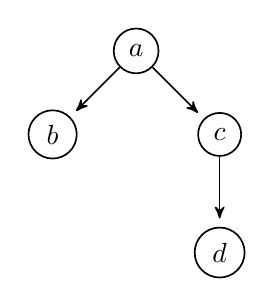
\begin{tikzpicture}[->,>=stealth',shorten >=3pt,auto,node distance=1.5cm,semithick]
    \tikzset{every state/.style={minimum size=0pt}}

    \node[state] (A)                    {$a$};
    \node[state] (B) [below left of=A] {$b$};
    \node[state] (C) [below right of=A]  {$c$};
    \node[state] (D) [below of=C] {$d$};

    \path (A) edge              node {} (B);
    \path (A) edge              node {} (C);
    \path (C) edge              node {} (D);
\end{tikzpicture}
\caption{A basic state transition system} 
\label{fig:basic_transition_system}
\end{figure}


We introduce the following auxiliary functions over states of a transition systems which will become 
useful in Section~\ref{sec:ctl_semantics} where we define the semantics of CTL operators in terms of transition systems.

\begin{definition}\label{def:pre}
    Let $\langle \Sigma, \tau \rangle$ be a transition system. The function $\text{pre} \colon \mathcal{P}(\Sigma) \to \mathcal{P}(\Sigma)$
    maps a set of states $X \in \mathcal{P}(\Sigma)$ to the set of their predecessors with respect to the program transition
    relation $\tau$:
\begin{equation}
    \text{pre}(X) \eqdef \{s \in \Sigma \ | \ \exists s' \in X \colon \langle s, s' \rangle \in \tau \}  
\end{equation}
\end{definition}


\begin{definition}\label{def:tilde_pre}
    Let $\langle \Sigma, \tau \rangle$ be a transition system. The function $\widetilde{\text{pre}} \colon \mathcal{P}(\Sigma) \to \mathcal{P}(\Sigma)$
    maps a set of states $X \in \mathcal{P}(\Sigma)$ to the set of their predecessors with respect to the program transition
    relation $\tau$ with the limitation that only those predecessor states are selected which exclusively transition to states in $X$:
\begin{equation}
    \widetilde{\text{pre}}(X) \eqdef \{s \in \Sigma \ | \ \forall s' \in X \colon \langle s, s' \rangle \in \tau \Rightarrow s' \in X \}  
\end{equation}
\end{definition}

To get an intuition for the difference between $\widetilde{\text{pre}}$ and $\text{pre}$, consider the state transition system 
depicted in Figure~\ref{fig:basic_transition_system}. There it holds that $\text{pre}(\{b, d\}) = \{a, c\}$ 
because $a$ is the predecessor of $b$ and $c$ the predecessor of $d$. 
However note that $\widetilde{\text{pre}}(\{b, d\}) = \{c\}$ since only $c$ has 
transitions that exclusively end up in either $b$ or $d$. 
Consequently it holds that $\widetilde{\text{pre}}(\{b, c\}) = \{a\}$ because $a$ transitions exclusively to either $b$ or $c$.\\

The next section introduces Computation Tree Logic, 
a logic for stating properties about transition systems.  

\section{Computation Tree Logic (CTL)}\label{sec:computation_tree_logic}

Computation Tree Logic (CTL) is a logic which allows stating properties about execution traces of state transition systems. 
In the context of this thesis, CTL is used to express temporal properties about the runtime behavior of programs. 
This section gives a brief introduction into the syntax and semantic of CTL.  
Further information about CTL can be found in~\cite{baier2008principles}.\\

We assume the existence of some atomic proposition logic over the set of states. 
Atomic propositions $a \in \mathtt{AP}$ state properties of states $\sigma \in \Sigma$. 
The satisfaction relation $\models \ \subseteq \Sigma \times \mathtt{AP}$ determines 
if a state satisfies an atomic proposition.


\subsection{Syntax}
The syntax of a CTL formula is given by the following grammar.

\begin{align*}
    \Phi  ::= \ & \\ 
    & a \ | \\
    & \neg \Phi \ | \ \Phi \land \Phi \ | \ \Phi \lor \Phi \ | \\
    & \forall\bigcirc\Phi \ | \ \exists\bigcirc\Phi \ | \\
    & \forall\lozenge\Phi \ | \ \exists\lozenge\Phi \ | \\
    & \forall\square\Phi \ | \ \exists\square\Phi \ | \\
    & \forall(\Phi \ U \ \Phi) | \ \exists(\Phi \ U \ \Phi) 
\end{align*}

The term $a$ is an atomic propositions. Formulae with quantifiers $\exists$ or $\forall$ are called
path-dependent, formulae without are called path-independent.

\subsection{Semantic}

We now define the satisfaction relation $\models$ between states $\sigma \in \Sigma$ and CTL formulae.
The satisfaction relation for atomic propositions $a \in \mathtt{AP}$ is assumed to be given by the underlying 
logic for atomic propositions.

\begin{align*}
    \sigma \models a  \iff &\sigma \models a \\ 
    \sigma \models \neg \Phi  \iff &\text{not} \ \sigma \models \Phi \\ 
    \sigma \models \Phi_1 \land \Phi_2   \iff &(\sigma \models \Phi_1) \ \text{and} \ (\sigma \models \Phi_1) \\ 
    \sigma \models \Phi_1 \lor \Phi_2   \iff &(\sigma \models \Phi_1) \ \text{or} \ (\sigma \models \Phi_1) \\ 
    \sigma \models \forall\bigcirc\Phi \iff  &\forall \pi \in Paths(\sigma) \colon (\pi [1] \models \Phi) \\ 
    \sigma \models \exists\bigcirc\Phi \iff  &\exists \pi \in Paths(\sigma) \colon (\pi [1] \models \Phi) \\ 
    \sigma \models \forall(\Phi_1 \ U \ \Phi_2) \iff &\forall \pi \in Paths(\sigma) \colon \\
    &(\exists j \geq 0 \colon \pi[j] \models \Phi_2 \land (\forall 0 \leq k < j \colon \pi[k] \models \Phi_1)) \\ 
    \sigma \models \exists(\Phi_1 \ U \ \Phi_2) \iff &\exists \pi \in Paths(\sigma) \colon\\
    &(\exists j \geq 0 \colon \pi[j] \models \Phi_2 \land (\forall 0 \leq k < j \colon \pi[k] \models \Phi_1)) \\ 
    \sigma \models \forall\square\Phi \iff  &\forall \pi \in Paths(\sigma) \colon (\forall j \geq 0 \colon \pi[j] \models \Phi) \\ 
    \sigma \models \exists\square\Phi \iff  &\exists \pi \in Paths(\sigma) \colon (\forall j \geq 0 \colon \pi[j] \models \Phi) \\ 
\end{align*}

The states $\sigma \in \Sigma$ are part of a state transition system $\langle \Sigma, \tau \rangle$ and 
$Paths(\sigma_0)$ is the set of all paths $\pi = \sigma_0 \sigma_1 \sigma_2 \dots$ starting from $\sigma_0$ with $\pi[j] = \sigma_j$.
The CTL formulae $\forall\lozenge\Phi$ and $\exists\lozenge\Phi$ are not explicitly defined. They are equivalent to 
$\forall(true \ U \ \Phi)$ and $\exists(true \ U \ \Phi)$. \\

Properties $\forall(\Phi_1 \ U \ \Phi_2)$ and $\exists(\Phi_1 \ U \ \Phi_2)$ are called \textsf{until} properties.
These properties require that a state satisfying $\Phi_2$ is reached eventually among all (some, respectively) paths, 
and until then $\Phi_1$ holds.\\

Properties $\forall\square\Phi$ and $\exists\square\Phi$ are called \textsf{global} properties. They state that all states among 
all (some, respectively) reachable paths satisfy the property $\Phi$.\\

Properties $\forall\bigcirc\Phi$ and $\exists\bigcirc\Phi$ are called \textsf{next} properties. They state that all (some, respectively) immediate next
states satisfy the property $\Phi$.\\

The following useful equivalence relations 
exists which can be used to relate existential to universal CTL formulae.

\begin{align*}
    \exists\bigcirc\Phi &\equiv \neg \forall\bigcirc(\neg \Phi)\\ 
    \exists\lozenge\Phi &\equiv \neg \forall\square(\neg \Phi) \\
    \exists\square\Phi  &\equiv \neg \forall\lozenge(\neg \Phi) \\
\end{align*}

The next section introduces the concept of ranking functions, a proof method for liveness properties. 
This proof method will then be extended to CTL in Section~\ref{sec:ctl_semantics}. 

\section{Ranking Functions}\label{sec:ranking_functions}

The traditional method for proving termination are \textit{ranking functions}~\cite{Touring49}~\cite{Floyd67}.
A ranking function is a partial function from program states to a well-ordered set like natural numbers or ordinals. 
To prove termination, the value of the ranking function must decrease during program execution. 
Cousot and Cousot prove the existence of a \textit{most precise ranking function} and that it can be derived 
by abstract interpretation \cite{CousotCousot-POPL12}. 
We will call this \textit{most precise ranking function}, as defined by Cousot and Cousot, 
the \textit{termination semantics} from now on.

\begin{definition}
    The \textit{termination semantics} is a ranking function 
    $\tau^{t} \in \Sigma \rightarrow \mathbb{O}$.
    A program starting from some initial state $\sigma \in \Sigma$ terminates if and only if $\sigma \in dom(\tau^{t})$.
\end{definition}

The \textit{termination semantics} assigns an upper bound on the number of steps until termination to each state. 
Therefore, a program terminates if its initial state is in the domain of the \textit{termination semantics}.\\

Based on the work of Cousot and Cousot~\cite{CousotCousot-POPL12}, Urban and Miné~\cite{UrbanM-VMCAI15} extended the 
\textit{termination semantics} to other liveness properties. More precisely to guarantee and recurrence properties. 
A guarantee property states that some state satisfying a given property is guaranteed to be reached eventually. 
Termination is therefore just a guarantee property stating that some final state will be eventually reached. 
As with termination, the \textit{guarantee semantics} is a ranking function that assigns each state an upper bound on the number of steps
until a state satisfying said property is reached. Guarantee properties can be expressed using the CTL formula $\forall\lozenge(a)$

\begin{definition}
    The \textit{guarantee semantics} is a ranking function 
    $\tau_{[S]}^{g} \in \Sigma \rightarrow \mathbb{O}$
    where $S \subseteq \Sigma$ is a set of states satisfying a desired property.
    A program starting from some state $\sigma \in \Sigma$ will reach a state 
    $s \in S$ if and only if $\sigma \in dom(\tau_{[S]}^{g})$.
\end{definition}

In addition to guarantee properties, Urban and Miné~\cite{UrbanM-VMCAI15} also introduced the \textit{recurrence semantics}.
A recurrence property guarantees that a program starting from some state $\sigma \in \Sigma$ will reach some state satisfying
a given property infinitely often. The value assigned to a state by the \textit{recurrence semantics}
is an upper bound on the number of executions steps until the next state satisfying the property is reached. 
Recurrence properties can be expressed using the CTL formula $\forall\square\forall\lozenge(a)$.

\begin{definition}
    The \textit{recurrence semantics} is a ranking function 
    $\tau_{[S]}^{r} \in \Sigma \rightarrow \mathbb{N}$
    where $S \subseteq \Sigma$ is a set of states satisfying a desired property.
    A program starting from some state $\sigma \in \Sigma$ will reach a state 
    $s \in S$ infinitely often if and only if $\sigma \in dom(\tau_{[S]}^{r})$.
\end{definition}

Figure~\ref{fig:ranking_functios_example} shows an example for the semantics discussed in this section.
We illustrate ranking functions by labeling the states with the corresponding value assigned to them by the function. 
The first example (a) shows the \textit{termination semantics} for a state transition system that always terminates. Therefore the initial state
has the value $2$ assigned to it stating that this program terminates in at most two steps.\\

The second example (b) shows the \textit{guarantee semantics} for the guarantee property that states that a gray state will be reached eventually 
($\forall\lozenge(\text{gray})$).
This holds for example (b), therefore the initial state has the value $2$ assigned to it. The program reaches a gray state in at most two steps.\\

The last example (c) shows the \textit{recurrence semantics} for the recurrence property that states that a gray state will be reached infinitely often
($\forall\square\forall\lozenge(\text{gray})$).
As one can see in the transition system, this is not true when starting from the initial state. Therefore the \textit{recurrence semantics} is undefined
for the initial state. However the property holds when starting from state $c$ or $d$. 
Accordingly these two states have the values $1$ and $0$ assigned to them.\\

We refer to~\cite{UrbanPhd} for a detailed discussion of the various semantics presented in this section.
The next section extends on the concepts of this section and presents a proof method for CTL properties.

\begin{figure}
    \begin{subfigure}[b]{0.32\textwidth}
        \centering
        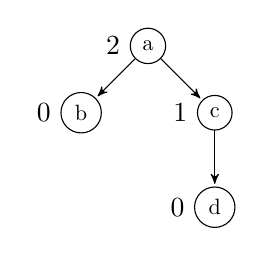
\begin{tikzpicture}[->,>=stealth',shorten >=1pt,node distance=1.5cm,thin]
            \tikzset{every state/.style={minimum size=0pt, scale=0.8}}
            \node[state, label=left:{2}] (A) {a};
            \node[state, label=left:{0}] (B) [below left of=A] {b};
            \node[state, label=left:{1}] (C) [below right of=A] {c};
            \node[state, label=left:{0}] (D) [below of=C] {d};
            \path (A) edge              node {} (B);
            \path (A) edge              node {} (C);
            \path (C) edge              node {} (D);
        \end{tikzpicture}
        \caption{$\tau^{t}$}
    \end{subfigure}
    \begin{subfigure}[b]{0.32\textwidth}
        \centering
        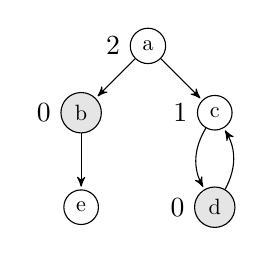
\begin{tikzpicture}[->,>=stealth',shorten >=1pt,node distance=1.5cm,thin]
            \tikzset{every state/.style={minimum size=0pt, scale=0.8}}
            \node[state, label=left:{2}] (A) {a};
            \node[state, fill=gray!20, label=left:{0}] (B) [below left of=A] {b};
            \node[state, label=left:{1}] (C) [below right of=A] {c};
            \node[state, fill=gray!20, label=left:{0}] (D) [below of=C] {d};
            \node[state] (E) [below of=B] {e};
            \path (A) edge              node {} (B);
            \path (A) edge              node {} (C);
            \path (C) edge[bend right]             node {} (D);
            \path (D) edge[bend right]              node {} (C);
            \path (B) edge              node {} (E);
        \end{tikzpicture}
        \caption{$\tau_{[\{b, d\}]}^{g}$}
    \end{subfigure}
    \begin{subfigure}[b]{0.32\textwidth}
        \centering
        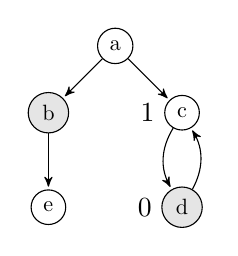
\begin{tikzpicture}[->,>=stealth',shorten >=1pt,node distance=1.5cm,thin]
            \tikzset{every state/.style={minimum size=0pt, scale=0.8}}
            \node[state] (A) {a};
            \node[state, fill=gray!20] (B) [below left of=A] {b};
            \node[state, label=left:{1}] (C) [below right of=A] {c};
            \node[state, fill=gray!20, label=left:{0}] (D) [below of=C] {d};
            \node[state] (E) [below of=B] {e};
            \path (A) edge              node {} (B);
            \path (A) edge              node {} (C);
            \path (C) edge[bend right]             node {} (D);
            \path (D) edge[bend right]              node {} (C);
            \path (B) edge              node {} (E);
        \end{tikzpicture}
        \caption{$\tau_{[\{b, d\}]}^{r}$}
    \end{subfigure}
    \caption{
        Example \textit{termination\ semantics} (a), 
        \textit{guarantee\ semantics} (b) and
        \textit{recurrence\ semantics} (c)
    } 
    \label{fig:ranking_functios_example}
\end{figure}


\section{Concrete Semantics for CTL}\label{sec:ctl_semantics}

In Section~\ref{sec:ranking_functions} we introduced the concept of ranking functions and explained how they express the semantics of 
termination and also liveness properties in general. We recall that ranking functions are a proof method for liveness properties. 
The ranking function assigns well-ordered values to program states. 
Liveness properties state that some goal state will be reached eventually. The ranking function assigns $0$ to those goal states 
and increased the values for states leading up to said goal state through backtracking.
One can determine if a state satisfies a liveness property by checking if the corresponding ranking function
assigns a value to said state. The assigned value is an upper bound on the number of steps until a goal state is reached.
In this section we extend this proof method presented in~\cite{UrbanPhd} to CTL.\\

CTL can define both liveness and safety properties. For liveness properties, ranking functions can be used as proof method. 
However, ranking functions are not suitable in the case of safety properties since there is no goal state to be reached eventually. 
Because a CTL formula can arbitrarily combine liveness and safety properties we will use a \textit{counting function} 
$\tau_\Phi \in \Sigma \rightarrow \mathbb{O}$ as proof method. 
The function $\tau_\Phi$ is similar to a ranking function, it assigns well-ordered values to states. 
A state satisfies a CTL property $\Phi$ if it is in the domain of $\tau_\Phi$. 
However, as opposed to ranking functions, the value of the \textit{counting function} $\tau_\Phi$ is not guaranteed to 
decrease. It will only decrease if $\Phi$ is a liveness property. 
In that case, the value of the function is an upper bound on the number of steps until some goal states is reached. 
Otherwise, in the case of safety properties, the value may be constant and is irrelevant. 
We call $\tau_\Phi$ the \textit{CTL semantics} from now on.

\begin{theorem}\label{thr:ctl_semantics}
    The \textit{CTL semantics} for a given CTL formula $\Phi$ is a counting function 
    $\tau_{\Phi} \in \Sigma \rightarrow \mathbb{N}$. 
    It encodes the semantics of $\Phi$ for a given state transition 
    system $\langle \Sigma, \tau \rangle$ such that 
    $\sigma \models \Phi \iff \sigma \in dom(\tau_{\Phi})$
\end{theorem}

We will define the \textit{CTL semantics} inductively for each CTL operator such that arbitrary 
combinations of CTL properties can be expressed.
Furthermore we split the definition into path-independent and path-dependent CTL operators. 

\subsection{Path Independent Operators}

We start by defining the \textit{CTL semantics} for atomic propositions and logic operators. 
These CTL properties are path independent and can be defined individually for each state $\sigma \in \Sigma$.
The definitions are formed according to Theorem~\ref{thr:ctl_semantics} and the 
satisfiability relation for CTL properties defined in Section~\ref{sec:computation_tree_logic}.\\

\begin{definition}\label{def:ctl_semantics_basic}
    Equations for path independent CTL operators
    \setlength{\jot}{15pt}
    \begin{align}
        \tau_a &\eqdef \lambda \sigma.
        \begin{cases}
            0                   & \text{if} \ \sigma \models a \\
            \text{undefined}    & \text{otherwise}
        \end{cases}\label{eq:ctl_atomic}\\
        %
        \tau_{\neg \Phi} &\eqdef \lambda \sigma.
        \begin{cases}
            0                   & \text{if} \ \sigma \notin dom(\tau_{\Phi}) \\
            \text{undefined}    & \text{otherwise}
        \end{cases}\label{eq:ctl_not}
        \\
        %
        \tau_{\Phi_1 \land \Phi_2} &\eqdef \lambda \sigma.
        \begin{cases}
            \sup\{\tau_{\Phi_1}(s), \tau_{\Phi_2}(\sigma)\} 
                                &\text{if } \sigma \in dom(\tau_{\Phi_1}) \cap dom(\tau_{\Phi_2}) \\
            \text{undefined}    & \text{otherwise}
        \end{cases}\label{eq:ctl_and}\\
        %
        \tau_{\Phi_1 \lor \Phi_2} &\eqdef \lambda \sigma.
        \begin{cases}
            \sup\{\tau_{\Phi_1}(\sigma), \tau_{\Phi_2}(\sigma)\}         & \text{if} \ \sigma \in dom(\tau_{\Phi_1}) \cap dom(\tau_{\Phi_2}) \\
            \tau_{\Phi_1}(\sigma)                                        & \text{if} \ \sigma \in dom(\tau_{\Phi_1}) \setminus dom(\tau_{\Phi_2}) \\
            \tau_{\Phi_2}(\sigma)                                        & \text{if} \ \sigma \in dom(\tau_{\Phi_2}) \setminus dom(\tau_{\Phi_1}) \\
            \text{undefined}    & \text{otherwise}
        \end{cases}\label{eq:ctl_or}
    \end{align}
\end{definition}

Equation~\ref{eq:ctl_atomic} assigns $0$ to all states that satisfy the atomic proposition $a$. 
In case of liveness properties, such as $\forall\lozenge a$, the value $0$ marks that the goal of the property has been reached. 
For safety properties, the value $0$ simply states that the states satisfies the property. \\

The logic $\neg$ operator in equation~\ref{eq:ctl_not} follows the same approach as for atomic propositions. 
It interprets $\neg \Phi$ as an atomic proposition and uses the fact that
$\sigma \notin dom(\tau_{\Phi}) \implies \sigma \models \neg \Phi$ which follows from Theorem~\ref{thr:ctl_semantics}.\\

The logical $\land$ and $\lor$ connectives in equations \ref{eq:ctl_and} and \ref{eq:ctl_or} reuse the values of the underlying functions $\tau_{\Phi_1}$ and
$\tau_{\Phi_2}$ according to the semantics of these operators. If a state is assigned a value by both functions, 
then the supremum of the two values is used. That way, if the two underlying properties $\Phi_1$ and $\Phi_2$ are liveness-properties,
we preserve the notion of increasing the values of the function when backtracking from the goal states of underlying properties.

\begin{lemma}\label{lem:ctl_semantics_path_independent}
    The \textit{CTL semantics} for path-independent CTL operators are sound and complete. 
    Let $\sigma \in \Sigma$ and $\Phi$, $\Phi_1$ and $\Phi_2$ be arbitrary CTL properties.
    \begin{align}
        \sigma \models a &\iff \sigma \in dom(\tau_{a})\\
        \sigma \models \neg \Phi &\iff \sigma \in dom(\tau_{\neg \Phi})\\
        \sigma \models \Phi_1 \land \Phi_2 &\iff \sigma \in dom(\tau_{\Phi_1 \land \Phi_2})\\
        \sigma \models \Phi_1 \lor \Phi_2 &\iff \sigma \in dom(\tau_{\Phi_1 \lor \Phi_2})
    \end{align}
\end{lemma}


\subsection{Path Dependent Operators}

\textit{CTL semantics} for path-dependent operators \textsf{until} and \textsf{global} are defined in terms of fixed-points. 
These fixed-points are defined over the partially ordered set of functions $\langle \Sigma \rightarrow \mathbb{N}, \sqsubseteq \rangle$. 
Fixed-point iterates are related to each other using the \textit{computational order} $\sqsubseteq$. 
This partial order relates functions in terms of expressiveness, i.e., for how many states can a function prove that the CTL property holds.

\begin{definition}\label{def:computational_order}
    Let $f, g \in \Sigma \rightarrow \mathbb{O}$. 
    The \textit{computational order} $\sqsubseteq$ is defined as follows.
    \begin{align*}
        f \sqsubseteq g \iff \text{dom}(f) \subseteq \text{dom}(g) \land \forall x \in \text{dom}(f): f(x) \leq g(x) \\
    \end{align*}
\end{definition}

The \textit{CTL semantics} are not computable in general. In Section~\ref{sec:abstract_ctl_semantics} we will present a sound decidable
abstraction of the \textit{CTL semantics}. Soundness is related to the \textit{approximation order} $\preceq$.

\begin{definition}\label{def:approximation_order}
    Let $f, g \in \Sigma \rightarrow \mathbb{O}$. 
    The \textit{approximation order} $\preceq$ is defined as follows.
    \begin{align*}
        f \preceq g \iff \text{dom}(f) \supseteq \text{dom}(g) \land \forall x \in \text{dom}(g): f(x) \leq g(x) \\
    \end{align*}
\end{definition}

The \textit{approximation order} ranks counting functions in terms of precision. A function $f$ is more precise than a function $g$ if
it is defined over more states than $g$ and if the value is smaller for all states in the domain of $g$. Intuitively, a more precise 
counting function is able to prove for more states that a CTL $\Phi$ holds or does not hold.

\subsubsection*{Until}

Recall that for the CTL property $\forall(\Phi_1 U \Phi_2)$ to hold for some state $\sigma \in \Sigma$, 
all paths starting from said state must form a chain of states satisfying $\Phi_1$ ending in a state satisfying $\Phi_2$. 
In case of $\exists(\Phi_1 U \Phi_2)$ at least on such path must exists.
The \textit{CTL semantics} for universal and existential \textsf{until} properties are defined as least fixed-points of the abstract transformers
\begin{align*}
\phi_{\forall(\Phi_1 U \Phi_2)} &\in (\Sigma \rightarrow \mathbb{N}) \rightarrow (\Sigma \rightarrow \mathbb{N}))\\
\phi_{\exists(\Phi_1 U \Phi_2)} &\in (\Sigma \rightarrow \mathbb{N}) \rightarrow (\Sigma \rightarrow \mathbb{N}))
\end{align*}

starting from the totally undefined counting function $\overset{.}{\emptyset}$.

\begin{definition}\label{def:ctl_semantics_until}
    \textit{CTL semantics} for existential and universal \textsf{until} properties
    \setlength{\jot}{15pt}
    \begin{align}
        \tau_{\forall(\Phi_1 U \Phi_2)}  &\eqdef \text{lfp}_{\overset{.}{\emptyset}}^{\sqsubseteq} \ \phi_{\forall(\Phi_1 U \Phi_2)}\\
        \phi_{\forall(\Phi_1 U \Phi_2)}f &\eqdef \lambda \sigma.
        \begin{cases}
            0                                                           
                & \text{if} \ \sigma \in dom(\tau_{\Phi_2}) \\
            \sup\{ f(\sigma') + 1 \ | \ \langle \sigma,\sigma' \rangle \in \tau \}    
                & \text{if} \ \sigma \notin dom(\tau_{\Phi_2}) \ \land \\ 
                & \sigma \in dom(\tau_{\Phi_1}) \ \land \\ 
                & \sigma \in \widetilde{pre}(dom(f)) \\
            \text{undefined}                                            
                & \text{otherwise}
        \end{cases}\\
        \tau_{\exists(\Phi_1 U \Phi_2)}  &\eqdef \text{lfp}_{\overset{.}{\emptyset}}^{\sqsubseteq} \ \phi_{\exists(\Phi_1 U \Phi_2)}\\
        \phi_{\exists(\Phi_1 U \Phi_2)}f &\eqdef \lambda \sigma.
        \begin{cases}
            0                                                           
                & \text{if} \ \sigma \in dom(\tau_{\Phi_2}) \\
            \sup\{ f(\sigma') + 1 \ | \ \langle \sigma,\sigma' \rangle \in \tau \}    
                & \text{if} \ \sigma \notin dom(\tau_{\Phi_2}) \ \land \\ 
                & \sigma \in dom(\tau_{\Phi_1}) \ \land \\ 
                & \sigma \in pre(dom(f)) \\
            \text{undefined}                                            
                & \text{otherwise}
        \end{cases}
    \end{align}
\end{definition}

This definition is a generalization of the \textit{guarantee semantics} presented in~\cite{UrbanM-VMCAI15}. 
The fixed-point iteration starts by assigning the value $0$ to all states that satisfy $\Phi_2$. 
In subsequent iterations we consider all states that satisfy $\Phi_1$ and from which one can only transition to states that already satisfy  
$\forall(\Phi_1 U \Phi_2)$. These states are then assigned the largest ranking value of all reachable states plus one. 
By performing iterations this way, we backtrack paths in the state transition systems that end in a state satisfying $\Phi_2$ and which are preceded by an 
unbroken chain of states satisfying $\Phi_1$. Every state on such a path is guaranteed to satisfy $\forall(\Phi_1 U \Phi_2)$. 
Furthermore, by starting from $0$ at states that satisfy $\Phi_2$ and incrementing the value of the function while backtracking, 
we construct a counting function such that the value assigned to each state is an 
upper bound on the number of steps until a state satisfying $\Phi_2$ is reached.\\

The $\widetilde{pre}$ relation guarantees that during the backtracking, only those states that
exclusively transition to states satisfying $\forall(\Phi_1 U \Phi_2)$, are considered. 
This condition can be relaxed for existential `until' properties by using the $pre$ relation instead. 
That way, states that have at least one reachable state satisfying $\exists(\Phi_1 U \Phi_2)$ are also considered 
during the backtracking (see Definitions~\ref{def:pre} and~\ref{def:tilde_pre}).\\

\begin{lemma}\label{lem:ctl_semantics_until}
    The \textit{CTL semantics} for \textsf{until} properties are sound and complete. 
    Let $\sigma \in \Sigma$ and $\Phi_1$, $\Phi_2$ be arbitrary CTL properties.
    \begin{align}
        \sigma \models \forall(\Phi_1 U \Phi_2) &\iff \sigma \in dom(\tau_{\forall(\Phi_1 U \Phi_2)})\\
        \sigma \models \exists(\Phi_1 U \Phi_2) &\iff \sigma \in dom(\tau_{\exists(\Phi_1 U \Phi_2)})
    \end{align}
\end{lemma}


Figures~\ref{fig:ctl_semantics_universal_until} and~\ref{fig:ctl_semantics_existential_until} give an example on how the
iterative computation for \textsf{until} properties works for universal and existential quantifiers. 
Note how Figure~\ref{fig:ctl_semantics_existential_until} has one additional iteration because of the existential quantifier. 
The initial state is added to the function in the last iteration because there exists one edge that leads to a state satisfying the property.  
For the universal property, the iteration stops after three iterations because not all successor states
of the initial state satisfy the property.


\begin{figure}
    \begin{subfigure}[b]{0.5\textwidth}
        \centering
        \resizebox{100pt}{!}{
            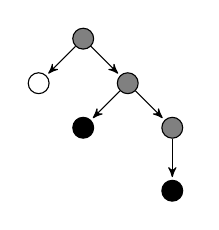
\begin{tikzpicture}[->,>=stealth',shorten >=1pt,auto,node distance=1cm,thin]
                \tikzset{every state/.style={minimum size=0pt, scale=0.8}}
                \node[state, fill=gray] (A) {};
                \node[state] (B) [below left of=A] {};
                \node[state, fill=gray] (C) [below right of=A] {};
                \node[state, fill=black] (D) [below left of=C] {};
                \node[state, fill=gray] (E) [below right of=C] {};
                \node[state, fill=black] (F) [below of=E] {};
                \path (A) edge              node {} (B);
                \path (A) edge              node {} (C);
                \path (C) edge              node {} (D);
                \path (C) edge              node {} (E);
                \path (E) edge              node {} (F);
            \end{tikzpicture}
        }
        \caption{Iteration 0}
    \end{subfigure}
    \begin{subfigure}[b]{0.5\textwidth}
        \centering
        \resizebox{100pt}{!}{
            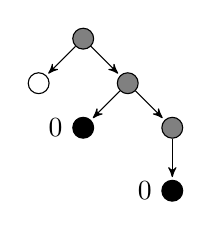
\begin{tikzpicture}[->,>=stealth',shorten >=1pt,auto,node distance=1cm,thin]
                \tikzset{every state/.style={minimum size=0pt, scale=0.8}}

                \node[state, fill=gray] (A) {};
                \node[state] (B) [below left of=A] {};
                \node[state, fill=gray] (C) [below right of=A] {};
                \node[state, fill=black, label=left:{0}] (D) [below left of=C] {};
                \node[state, fill=gray] (E) [below right of=C] {};
                \node[state, fill=black, label=left:{0}] (F) [below of=E] {};

                \path (A) edge              node {} (B);
                \path (A) edge              node {} (C);
                \path (C) edge              node {} (D);
                \path (C) edge              node {} (E);
                \path (E) edge              node {} (F);
            \end{tikzpicture}
        }
        \caption{Iteration 1}
    \end{subfigure}
    \par\bigskip
    \begin{subfigure}[b]{0.5\textwidth}
        \centering
        \resizebox{100pt}{!}{
            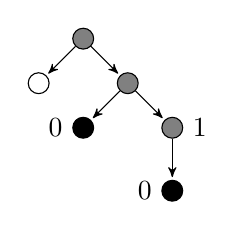
\begin{tikzpicture}[->,>=stealth',shorten >=1pt,auto,node distance=1cm,thin]
                \tikzset{every state/.style={minimum size=0pt, scale=0.8}}

                \node[state, fill=gray] (A) {};
                \node[state] (B) [below left of=A] {};
                \node[state, fill=gray] (C) [below right of=A] {};
                \node[state, fill=black, label=left:{0}] (D) [below left of=C] {};
                \node[state, fill=gray, label=right:{1}] (E) [below right of=C] {};
                \node[state, fill=black, label=left:{0}] (F) [below of=E] {};

                \path (A) edge              node {} (B);
                \path (A) edge              node {} (C);
                \path (C) edge              node {} (D);
                \path (C) edge              node {} (E);
                \path (E) edge              node {} (F);
            \end{tikzpicture}
        }
        \caption{Iteration 2}
    \end{subfigure}
    \begin{subfigure}[b]{0.5\textwidth}
        \centering
        \resizebox{100pt}{!}{
            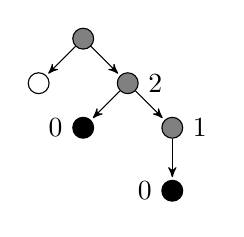
\begin{tikzpicture}[->,>=stealth',shorten >=1pt,auto,node distance=1cm,thin]

                \tikzset{every state/.style={minimum size=0pt, scale=0.8}}

                \node[state, fill=gray] (A) {};
                \node[state] (B) [below left of=A] {};
                \node[state, fill=gray, label=right:{2}] (C) [below right of=A] {};
                \node[state, fill=black, label=left:{0}] (D) [below left of=C] {};
                \node[state, fill=gray, label=right:{1}] (E) [below right of=C] {};
                \node[state, fill=black, label=left:{0}] (F) [below of=E] {};

                \path (A) edge              node {} (B);
                \path (A) edge              node {} (C);
                \path (C) edge              node {} (D);
                \path (C) edge              node {} (E);
                \path (E) edge              node {} (F);
            \end{tikzpicture}
        }
        \caption{Iteration 3}
    \end{subfigure}
    \caption{Iterative computation of $\tau_{\forall(gray \ U \ black)}$.} 
    \label{fig:ctl_semantics_universal_until}
\end{figure}




\begin{figure}
    \begin{subfigure}[b]{0.5\textwidth}
        \centering
        \resizebox{100pt}{!}{
            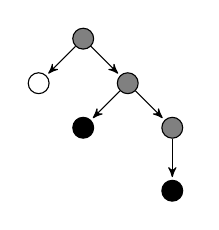
\begin{tikzpicture}[->,>=stealth',shorten >=1pt,auto,node distance=1cm,thin]
                \tikzset{every state/.style={minimum size=0pt, scale=0.8}}
                \node[state, fill=gray] (A) {};
                \node[state] (B) [below left of=A] {};
                \node[state, fill=gray] (C) [below right of=A] {};
                \node[state, fill=black] (D) [below left of=C] {};
                \node[state, fill=gray] (E) [below right of=C] {};
                \node[state, fill=black] (F) [below of=E] {};
                \path (A) edge              node {} (B);
                \path (A) edge              node {} (C);
                \path (C) edge              node {} (D);
                \path (C) edge              node {} (E);
                \path (E) edge              node {} (F);
            \end{tikzpicture}
        }
        \caption{Iteration 0}
    \end{subfigure}
    \begin{subfigure}[b]{0.5\textwidth}
        \centering
        \resizebox{100pt}{!}{
            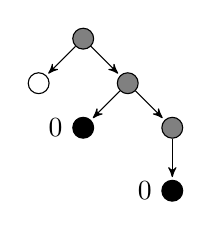
\begin{tikzpicture}[->,>=stealth',shorten >=1pt,auto,node distance=1cm,thin]
                \tikzset{every state/.style={minimum size=0pt, scale=0.8}}

                \node[state, fill=gray] (A) {};
                \node[state] (B) [below left of=A] {};
                \node[state, fill=gray] (C) [below right of=A] {};
                \node[state, fill=black, label=left:{0}] (D) [below left of=C] {};
                \node[state, fill=gray] (E) [below right of=C] {};
                \node[state, fill=black, label=left:{0}] (F) [below of=E] {};

                \path (A) edge              node {} (B);
                \path (A) edge              node {} (C);
                \path (C) edge              node {} (D);
                \path (C) edge              node {} (E);
                \path (E) edge              node {} (F);
            \end{tikzpicture}
        }
        \caption{Iteration 1}
    \end{subfigure}
    \par\bigskip
    \begin{subfigure}[b]{0.32\textwidth}
        \centering
        \resizebox{100pt}{!}{
            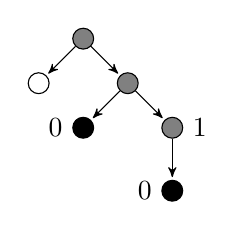
\begin{tikzpicture}[->,>=stealth',shorten >=1pt,auto,node distance=1cm,thin]
                \tikzset{every state/.style={minimum size=0pt, scale=0.8}}

                \node[state, fill=gray] (A) {};
                \node[state] (B) [below left of=A] {};
                \node[state, fill=gray] (C) [below right of=A] {};
                \node[state, fill=black, label=left:{0}] (D) [below left of=C] {};
                \node[state, fill=gray, label=right:{1}] (E) [below right of=C] {};
                \node[state, fill=black, label=left:{0}] (F) [below of=E] {};

                \path (A) edge              node {} (B);
                \path (A) edge              node {} (C);
                \path (C) edge              node {} (D);
                \path (C) edge              node {} (E);
                \path (E) edge              node {} (F);
            \end{tikzpicture}
        }
        \caption{Iteration 2}
    \end{subfigure}
    \begin{subfigure}[b]{0.32\textwidth}
        \centering
        \resizebox{100pt}{!}{
            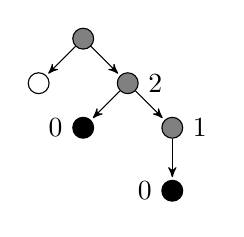
\begin{tikzpicture}[->,>=stealth',shorten >=1pt,auto,node distance=1cm,thin]

                \tikzset{every state/.style={minimum size=0pt, scale=0.8}}

                \node[state, fill=gray] (A) {};
                \node[state] (B) [below left of=A] {};
                \node[state, fill=gray, label=right:{2}] (C) [below right of=A] {};
                \node[state, fill=black, label=left:{0}] (D) [below left of=C] {};
                \node[state, fill=gray, label=right:{1}] (E) [below right of=C] {};
                \node[state, fill=black, label=left:{0}] (F) [below of=E] {};

                \path (A) edge              node {} (B);
                \path (A) edge              node {} (C);
                \path (C) edge              node {} (D);
                \path (C) edge              node {} (E);
                \path (E) edge              node {} (F);
            \end{tikzpicture}
        }
        \caption{Iteration 3}
    \end{subfigure}
    \begin{subfigure}[b]{0.32\textwidth}
        \centering
        \resizebox{100pt}{!}{
            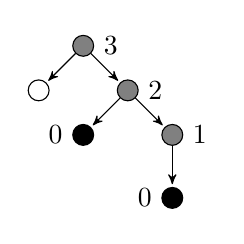
\begin{tikzpicture}[->,>=stealth',shorten >=1pt,auto,node distance=1cm,thin]

                \tikzset{every state/.style={minimum size=0pt, scale=0.8}}

                \node[state, fill=gray, label=right:{3}] (A) {};
                \node[state] (B) [below left of=A] {};
                \node[state, fill=gray, label=right:{2}] (C) [below right of=A] {};
                \node[state, fill=black, label=left:{0}] (D) [below left of=C] {};
                \node[state, fill=gray, label=right:{1}] (E) [below right of=C] {};
                \node[state, fill=black, label=left:{0}] (F) [below of=E] {};

                \path (A) edge              node {} (B);
                \path (A) edge              node {} (C);
                \path (C) edge              node {} (D);
                \path (C) edge              node {} (E);
                \path (E) edge              node {} (F);
            \end{tikzpicture}
        }
        \caption{Iteration 4}
    \end{subfigure}
    \caption{Iterative computation of $\tau_{\exists(gray \ U \ black)}$.} 
    \label{fig:ctl_semantics_existential_until}
\end{figure}


\subsubsection*{Global}

Recall that the CTL \textsf{global} operator states that some property must hold globally, i.e., indefinitely for 
\textit{all} paths starting from some state in the case of the universal
quantifier ($\forall\square\Phi$) or for \textit{some} paths in case of the existential quantifier ($\exists\square\Phi$). 
The CTL semantics for \textsf{global} properties are defined as greatest fixed-point of the abstract transformers
\begin{align*}
    \phi_{\forall(\Phi_1 U \Phi_2)} \in (\Sigma \rightarrow \mathbb{N}) \rightarrow (\Sigma \rightarrow \mathbb{N}))\\
    \phi_{\exists(\Phi_1 U \Phi_2)} \in (\Sigma \rightarrow \mathbb{N}) \rightarrow (\Sigma \rightarrow \mathbb{N}))
\end{align*}
starting from the CTL semantics $\tau_\Phi$ of the inner CTL property.

\begin{definition}\label{def:ctl_semantics_global}
    Equations for CTL global operator
    \setlength{\jot}{15pt}
    \begin{align}
        \tau_{\forall\square\Phi} &\eqdef \text{gfp}_{\tau_\Phi}^{\sqsubseteq} \  \phi_{\forall\square\Phi}\\
        \phi_{\forall\square\Phi}f &\eqdef \lambda \sigma.
        \begin{cases}
            f(x)                            & \text{if} \ \sigma \in \widetilde{pre}(dom(f)) \\
            \text{undefined}                & \text{otherwise}
        \end{cases}\\
        \tau_{\exists\square\Phi} &\eqdef \text{gfp}_{\tau_\Phi}^{\sqsubseteq} \  \phi_{\exists\square\Phi}\\
        \phi_{\exists\square\Phi}f &\eqdef \lambda \sigma.
        \begin{cases}
            f(x)                            & \text{if} \ \sigma \in pre(dom(f)) \\
            \text{undefined}                & \text{otherwise}
        \end{cases}
    \end{align}
\end{definition}

This definition is based on the \textit{recurrence semantics} presented in~\cite{UrbanM-VMCAI15}.
As with the \textsf{until} operator, we distinguish between universal and existential properties by using either $\widetilde{pre}$ or $pre$. 
The fixed-point iteration starts with the counting function $\tau_\Phi$ of the inner property $\Phi$.
At each iteration, every state that is still part of the domain of the function is inspected. 
The inspected state is kept in the domain of the function if \textit{all} its successor states 
(or \textit{some} for the existential case) are also part of the domain of the function, otherwise it is removed.
That way, only states which are part of an infinite path consisting exclusively of states satisfying $\Phi$ are kept in 
the domain of the function.

\begin{lemma}\label{lem:ctl_semantics_global}
    The \textit{CTL semantics} for \textsf{global} properties are sound and complete. 
    Let $\sigma \in \Sigma$ and $\Phi$ be an arbitrary CTL property.
    \begin{align}
        \sigma \models \forall\square\Phi &\iff \sigma \in dom(\tau_{\forall\square\Phi})\\
        \sigma \models \exists\square\Phi &\iff \sigma \in dom(\tau_{\exists\square\Phi})
    \end{align}
\end{lemma}



Figures~\ref{fig:ctl_semantics_universal_global} and~\ref{fig:ctl_semantics_existential_global} show this for 
$\tau_{\exists\square\Phi}$ and $\tau_{\forall\square\Phi}$. Both iterations start with some initial counting function $\tau_\Phi$.
In the first iteration state $b$ is removed because it has no outgoing edges. For the existential case, the iteration stops here because
all remaining states $a$, $c$ and $d$ have at least one edge to a node that is part of the function. In the universal case we get an additional
iteration that removes state $a$ because not all of its successor nodes (namely $b$) are part of the function. 
Note that only infinite paths are considered to hold globally. 


\begin{figure}

    \begin{subfigure}[b]{0.32\textwidth}
        \centering
        \resizebox{100pt}{!}{
            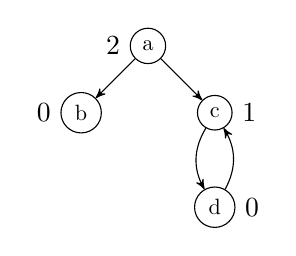
\begin{tikzpicture}[->,>=stealth',node distance=1.5cm,thin]
                \tikzset{every state/.style={minimum size=0pt, scale=0.8}}
                \node[state, label=left:{2}] (A) {a};
                \node[state, label=left:{0}] (B) [below left of=A] {b};
                \node[state, label=right:{1}] (C) [below right of=A] {c};
                \node[state, label=right:{0}] (E) [below of=C] {d};
                \path (A) edge              node {} (B);
                \path (A) edge              node {} (C);
                \path (C) edge[bend right]              node {} (E);
                \path (E) edge[bend right]              node {} (C);
            \end{tikzpicture}
        }
        \caption{Iteration 0}
    \end{subfigure}
    \begin{subfigure}[b]{0.32\textwidth}
        \centering
        \resizebox{100pt}{!}{
            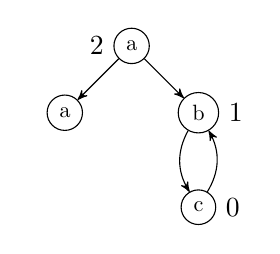
\begin{tikzpicture}[->,>=stealth',node distance=1.5cm,thin]
                \tikzset{every state/.style={minimum size=0pt, scale=0.8}}
                \node[state, label=left:{2}] (A) {a};
                \node[state, label=left:{}] (B) [below left of=A] {a};
                \node[state, label=right:{1}] (C) [below right of=A] {b};
                \node[state, label=right:{0}] (E) [below of=C] {c};
                \path (A) edge              node {} (B);
                \path (A) edge              node {} (C);
                \path (C) edge[bend right]              node {} (E);
                \path (E) edge[bend right]              node {} (C);
            \end{tikzpicture}
        }
        \caption{Iteration 1}
    \end{subfigure}
    \begin{subfigure}[b]{0.32\textwidth}
        \centering
        \resizebox{100pt}{!}{
            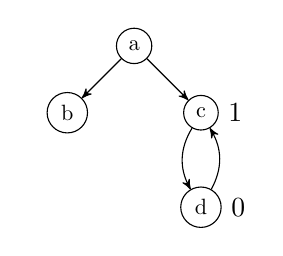
\begin{tikzpicture}[->,>=stealth',node distance=1.5cm,thin]
                \tikzset{every state/.style={minimum size=0pt, scale=0.8}}
                \node[state, label=left:{}] (A) {a};
                \node[state, label=left:{}] (B) [below left of=A] {b};
                \node[state, label=right:{1}] (C) [below right of=A] {c};
                \node[state, label=right:{0}] (E) [below of=C] {d};
                \path (A) edge              node {} (B);
                \path (A) edge              node {} (C);
                \path (C) edge[bend right]              node {} (E);
                \path (E) edge[bend right]              node {} (C);
            \end{tikzpicture}
        }
        \caption{Iteration 2}
    \end{subfigure}
    \caption{Iterative computation of $\tau_{\forall\square\Phi}$.} 
    \label{fig:ctl_semantics_universal_global}
\end{figure}

\begin{figure}
    \begin{subfigure}[b]{0.5\textwidth}
        \centering
        \resizebox{100pt}{!}{
            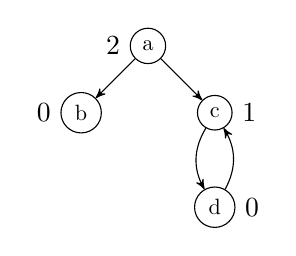
\begin{tikzpicture}[->,>=stealth',node distance=1.5cm,thin]
                \tikzset{every state/.style={minimum size=0pt, scale=0.8}}
                \node[state, label=left:{2}] (A) {a};
                \node[state, label=left:{0}] (B) [below left of=A] {b};
                \node[state, label=right:{1}] (C) [below right of=A] {c};
                \node[state, label=right:{0}] (E) [below of=C] {d};
                \path (A) edge              node {} (B);
                \path (A) edge              node {} (C);
                \path (C) edge[bend right]              node {} (E);
                \path (E) edge[bend right]              node {} (C);
            \end{tikzpicture}
        }
        \caption{Iteration 0}
    \end{subfigure}
    \begin{subfigure}[b]{0.5\textwidth}
        \centering
        \resizebox{100pt}{!}{
            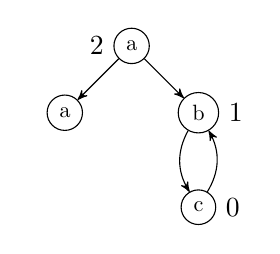
\begin{tikzpicture}[->,>=stealth',node distance=1.5cm,thin]
                \tikzset{every state/.style={minimum size=0pt, scale=0.8}}
                \node[state, label=left:{2}] (A) {a};
                \node[state, label=left:{}] (B) [below left of=A] {a};
                \node[state, label=right:{1}] (C) [below right of=A] {b};
                \node[state, label=right:{0}] (E) [below of=C] {c};
                \path (A) edge              node {} (B);
                \path (A) edge              node {} (C);
                \path (C) edge[bend right]              node {} (E);
                \path (E) edge[bend right]              node {} (C);
            \end{tikzpicture}
        }
        \caption{Iteration 1}
    \end{subfigure}
    \caption{Iterative computation of $\tau_{\exists\square\Phi}$.} 
    \label{fig:ctl_semantics_existential_global}
\end{figure}


\subsubsection*{Next}

The \textsf{next} operator is path dependent but does not require fixed-point iterations. 
A state satisfies $\forall\bigcirc\Phi$ if all its immediate successors satisfy the property $\Phi$,
correspondingly $\exists\bigcirc\Phi$ is satisfied if at least one immediate successor satisfies the property $\Phi$. 
This corresponds to the definition of the $\widetilde{pre}$ and $pre$ relations. Zero is assigned to each state
that satisfies the property to construct a valid counting function according to Theorem~\ref{thr:ctl_semantics}.

\begin{definition}\label{def:ctl_semantics_next}
    Equations for CTL next operator
    \setlength{\jot}{15pt}
    \begin{align}
        \tau_{\forall\bigcirc\Phi} &\eqdef \lambda \sigma.
        \begin{cases}
            0                   & \text{if} \ \sigma \in \widetilde{pre}(dom(\tau_\Phi)) \\
            \text{undefined}    & \text{otherwise}
        \end{cases}\\
        \tau_{\exists\bigcirc\Phi} &\eqdef \lambda \sigma.
        \begin{cases}
            0                   & \text{if} \ \sigma \in pre(dom(\tau_\Phi)) \\
            \text{undefined}    & \text{otherwise}
        \end{cases}
    \end{align}
\end{definition}

\begin{lemma}\label{lem:ctl_semantics_next}
    The \textit{CTL semantics} for \textsf{next} properties are sound and complete. 
    Let $\sigma \in \Sigma$ and $\Phi$ be an arbitrary CTL property.
    \begin{align}
        \sigma \models \forall\bigcirc\Phi &\iff \sigma \in dom(\tau_{\forall\bigcirc\Phi})\\
        \sigma \models \exists\bigcirc\Phi &\iff \sigma \in dom(\tau_{\exists\bigcirc\Phi})
    \end{align}
\end{lemma}


\section{Imperative Language}\label{sec:imperative_language}

In this section we briefly introduce a minimal imperative programming language. 
It will be used in Section~\ref{sec:abstract_ctl_semantics} to define the abstract CTL semantics.
The language has no procedures, pointers or recursion and is non-deterministic.
Variables are integer valued and statically allocated. We chose a simple language to 
keep the definitions of the abstract CTL semantics simple and concise. 
However, the implementation of our static analyzer 
will support a more feature-rich programming language (see Section~\ref{sec:implementation}).\\

First we define the syntax for arithmetic and boolean expressions. 
The syntax definitions are based on Chapter 3 of~\cite{UrbanPhd}.

\begin{definition}\label{def:arith_bool_syntax}
    Syntax for arithmetic and boolean expressions. \\
    Arithmetic expressions are defined over a set of variables $\mathcal{X}$.
    \begin{align*}
        \setlength{\jot}{15pt}
        aexp \ ::= \ & \ \ X && X \in \mathcal{X} \\
        &| \  [i_1, i_2] && i_1 \in \mathbb{Z} \cup \{ -\infty \},\ i_1 \in \mathbb{Z} \cup \{\infty \},\ i_1 \leq i_2  \\
        &| \  - aexp \\
        &| \  aexp \diamond aexp && \diamond \in \{ +, -, *, / \}\\
        \\
        bexp \ ::= \ & \ \ ?  && \text{non-deterministic choice} \\
        &| \  \neg bexp \\
        &| \  bexp \land bexp \\
        &| \  bexp \lor bexp \\
        &| \  aexp \diamond aexp && \diamond \in \{<, \leq, >, \geq \}\\
    \end{align*}
\end{definition}

The semantics for expressions are defined as expected. 
Please refer to~\cite{UrbanPhd} for a formal definition. 
Note that the symbol $?$ stands for non-deterministic choice.\\

Programs are defined in terms of control-flow-graphs. The control-flow-graph of a program models all possible program executions as
paths in the graph.

\begin{definition}\label{def:control_flow_graph}
    \textbf{Program representation as control-flow-graph.}
    A control-flow-graph is a tuple $(\mathcal{L}, E)$.
    $\mathcal{L}$ is the set of program labels, also called nodes. 
    $E \subseteq (\mathcal{L} \times stmt \times \mathcal{L})$ is the set of edges in the control-flow-graph where
    $stmt$ is the set of all program statements.
    \begin{align*}
        \setlength{\jot}{15pt}
        stmt \ ::= \ & \ \ \mathtt{skip} \\
        &| \ bexp \\
        &| \ X := aexp  && X \in \mathcal{X} \\
    \end{align*}
\end{definition}

Every control point of a program is assigned a label $l \in \mathcal{L}$. 
The nodes in the control-flow-graph correspond to those labels. 
An edge $(u, s, v) \in E$ states that one can transition from node
$u$ to $v$ by executing statement $s$. 
The \texttt{skip} statement transitions from one node to another without doing anything, 
the boolean expression $bexp$ limits the set of states
that are allowed to transition to the next node to the one satisfying $bexp$ and the assignment $X := aexp$ assigns the value of the arithmetic expression $aexp$
to the variable $X$. A program consists of a control-flow-graph and two special labels 
$l_{entry}$ and $l_{exit}$ that denote the program entry and exit point.\\

We introduce the following auxiliary functions on nodes of a control-flow-graph to 
refer to the incoming and outgoing edges of a node.

\begin{definition}\label{def:cfg_in}
    Given a control-flow-graph $(\mathcal{L}, E)$ and some node $l \in \mathcal{L}$
    \begin{align*}
        in(l) &\eqdef \{(u, s, v) \in E \ | \ v = l \}\\
        out(l) &\eqdef \{(u, s, v) \in E \ | \ u = l \}\\
    \end{align*}
\end{definition}


\section{Decision Tree Abstract Domain}\label{sec:decision_tree_abstract_domain}

This section briefly recaps the decision tree abstract domain~\cite{UrbanPhd}. 
Decision trees encode piecewise-defined linear functions which are used as an abstraction 
of the counting functions introduced in Section~\ref{sec:ranking_functions}. 
First we give a description of the decision tree abstract domain. 
Then we introduce ordering relations between the elements of the domain and relevant operations on the elements of the domain. 
An in-depth description of the topics covered in this section can be found in~\cite{UrbanPhd}.\\

\subsection{Domain}

The elements of the abstract domain are binary decision trees. The nodes of the trees are linear constraints and the leafs are linear functions
of the program variables. Decision trees partition the state space, given by a set of variables $\mathcal{X}$, into partitions. 
Each partition is defined through the conjunction of linear constraints on the path from root to leaf in the decision tree.
The linear function at the leaf determines the value of the function for the corresponding partition of the state space.\\

\begin{figure}
    \centering
    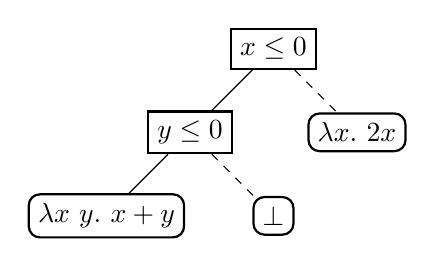
\begin{tikzpicture}[node distance=1.5cm]
        \tikzset{
            inner_node/.style={draw, shape = rectangle, thick},
            leaf/.style={draw, shape = rectangle, rounded corners, thick}
        }
        \node[inner_node] (A) {$x \leq 0$};
        \node[inner_node] (B) [below left of= A] {$y \leq 0$};
        \node[leaf] (C) [below right of= A] {$\lambda x.\ 2x$};
        \node[leaf] (D) [below left of= B] {$\lambda x \ y. \ x + y$};
        \node[leaf] (E) [below right of= B] {$\bot$};
        \path (A) edge              node {} (B);
        \path (A) edge [dashed]              node {} (C);
        \path (B) edge               node {} (D);
        \path (B) edge [dashed]              node {} (E);
    \end{tikzpicture}
    \caption{Example for decision tree}
    \label{fig:decision_tree_example}
\end{figure}

Figure~\ref{fig:decision_tree_example} gives an example for such a decision tree. 
It consists of two nodes with linear constraints $x \leq 0$ and $y \leq 0$. The left most leaf is the function $\lambda x \ y. \ x + y$. 
It is defined for all states satisfying $x \leq 0 \land y \leq 0$ according to the constraints from root to leaf. 
The right most leaf is the function $\lambda x.\ 2x$, it is defined for all states satisfying $\neg (x \leq 0)$ 
(following the right child of a node negates the linear constraint). The leaf in the middle is a bottom node, 
signifying that the function for the corresponding partition is undefined. 
In summary the decision tree in Figure~\ref{fig:decision_tree_example} is equivalent to the following partial function:

\[
    f(x, y) = \begin{cases}
            x+y                   & \text{if} \ x \leq 0 \land y \leq 0 \\
            2x                   & \text{if} \ x > 0 \\
            \text{undefined}    & \text{otherwise}
        \end{cases}
\]

We will now formalize the decision tree abstract domain.

\subsubsection*{Constraints}

The constrains at the inner nodes of the decision tree are elements of the 
\textit{linear constraints auxiliary abstract domain} $\mathcal{C}$.  

\[
    \mathcal{C} \eqdef 
    \left
        \{ 
        c_1 X_1 + \dots + c_n X_n + c_{n+1} \geq 0 \
        \middle\vert 
        \begin{array}{l}
            \mathcal{X} = \{X_1, \dots, X_n\}\\
            c_1, \dots, c_n, c_{n+1} \in \mathbb{Z} \\
            gcd(|c_1|, \dots, |c_n|, |c_{n+1}|) = 1
        \end{array}
    \right
    \}
\]

Elements of $\mathcal{C}$ can be instances of the \textit{interval abstract domain}~\cite{CousotCousot76-1}, 
the \textit{octagon abstract domain}~\cite{Mine:2006:OAD:1145489.1145526} or the \textit{polyhedra abstract domain}~\cite{Cousot:1978:ADL:512760.512770}.

\subsubsection*{Functions}

Leafs of the decision trees are elements of the \textit{functions auxiliary abstract domain} $\mathcal{F}$.
Elements of $\mathcal{F}$ are either natural valued linear functions or one of the two special elements $\top_{\mathcal{F}}$ or $\bot_{\mathcal{F}}$.
The element $\bot_{\mathcal{F}}$ indicates that the function is undefined on the given partition. 
The element $\top_{\mathcal{F}}$ indicates that the value of the function is unknown for the given partition.
\[
    \mathcal{F} \eqdef \{ \mathbb{Z}^{|\mathcal{X}|} \rightarrow \mathbb{N} \} \cup \{ \top_{\mathcal{F}}, \ \bot_{\mathcal{F}} \}
\]
We will write constant functions that return a value $n \in \mathbb{N}$ by just stating the constant value, e.g., $0 \in \mathcal{F}$ 
denotes the constant function that returns $0$ for every state.\\

In the following sections we will distinguish between so called \textit{defined} and \textit{undefined} leafs. 
A leaf $f \in \mathcal{F}$ is called \textit{defined} if $f$ is neither $\top_{\mathcal{F}}$ nor $\bot_{\mathcal{F}}$  and \textit{undefined} otherwise.
Defined leafs assign an actual value to its partition, therefore the function that the decision tree represents is defined for that partition. Otherwise 
the function is undefined.


\subsubsection*{Decision Trees}

We now define the decision tree abstract domain $\mathcal{T}$.
An element $t \in \mathcal{T}$ is either a \textit{leaf node} $\mathtt{LEAF} \colon f$ consisting of a function $f \in \mathcal{F}$ (denoted $t.f$),
or a \textit{decision node} $\mathtt{NODE}\{c\}: l; r$ consists of a linear constraint $c \in \mathcal{C}$ (denoted $t.c$) 
and a left and a right sub tree $l, r \in \mathcal{T}$ 
(denoted $t.l$ and $t.r$).
\[
    \mathcal{T} \eqdef \{\mathtt{LEAF} \colon f \ | \ f \in \mathcal{F}\} \cup \{\mathtt{NODE}\{c\}: l; r \ | \ c \in \mathcal{C}, l, r \in \mathcal{T} \} 
\]

For algorithmic purposes we also define $\mathcal{T}_{\mathtt{NIL}}$. 
This adds an additional leaf element \texttt{NIL} to $\mathcal{T}$ to represent the absence of information about a partition.
\texttt{NIL} leafs usually appear if a partition in a decision tree can be excluded because it is infeasible w.r.t.\ the program execution.
\[
    \mathcal{T}_{\mathtt{NIL}} \eqdef \{\mathtt{NIL}\} \ \cup \ \{\mathtt{LEAF} \colon f \ | 
    \ f \in \mathcal{F}\} \ \cup \ \{\mathtt{NODE}\{c\}: l; r \ | \ c \in \mathcal{C}, l, r \in \mathcal{T}_{\mathtt{NIL}}  \} 
\]


\subsubsection*{Sound Abstractions}

Decision trees are an abstraction of counting functions.  
A sound abstraction is defined in terms of the \textit{approximation order} $\preceq$ (see Definition~\ref{def:approximation_order}).\\

\begin{definition}\label{def:sound_abstraction}
    Let $\gamma \in \mathcal{T} \rightarrow (\Sigma \rightarrow \mathbb{O}) $ be the concretization function from decision trees to counting functions.
    A decision tree $t \in \mathcal{T}$ is a sound abstraction of a counting function $f \in \Sigma \rightarrow \mathbb{N}$ if $f \preceq \gamma(t)$.\\
\end{definition}

This definitions allows us to soundly define computable abstractions of counting functions. 
Every decision tree computed in such a way captures the behavior of the concrete counting function for 
all defined partitions of the tree.

\subsubsection*{Orders}

We now define the 
\textit{computational order} $\sqsubseteq_{\mathcal{T}}$ and \textit{approximation order} $\preceq_{\mathcal{T}}$
over elements of $\mathcal{T}$. These orders are an approximation of the corresponding orders presented in 
Section~\ref{sec:ctl_semantics} (see Definitions~\ref{def:computational_order} and~\ref{def:approximation_order}).\\

Both orders are defined by leaf-wise comparison of two decision trees. To that end we define the   
\textit{computational order} $\sqsubseteq_{\mathcal{F}}$ and \textit{approximation order} $\preceq_{\mathcal{F}}$
for elements of $\mathcal{F}$. Two trees are related to each other if all leafs 
are pairwise related w.r.t. $\sqsubseteq_{\mathcal{F}}$ ($\preceq_{\mathcal{F}}$, respectively). 
Please refer to~\cite{UrbanPhd} for a detailed explanation.\\

The two orders $\sqsubseteq_{\mathcal{F}}$ and $\preceq_{\mathcal{F}}$ are identical for function values 
$f \in \mathbb{Z}^{|\mathcal{X}|} \rightarrow \mathbb{N}$.
Pairings with the special elements $\top_{\mathcal{F}}$ and $\bot_{\mathcal{F}}$ are related to each other according to the
Hasse diagrams in Figure~\ref{fig:function_comp_approx_hasse}. 

\begin{definition}\label{def:fun_comp_approx_order}
    The \textit{computation order} $\sqsubseteq_{\mathcal{F}}$ and \textit{approximation order} $\preceq_{\mathcal{F}}$
    for elements  $f_1, f_2 \in \mathcal{F} \setminus \{\top_{\mathcal{F}}, \ \bot_{\mathcal{F}} \} $ are defined as follows.
    \begin{align*}
        f_1 \sqsubseteq_{\mathcal{F}} f_2  \iff  f_1 \preceq_{\mathcal{F}} f_2 \iff
        \forall x \in \mathbb{Z}^{|\mathcal{X}|} \colon f_1(x) \leq f_2(x)
    \end{align*}
\end{definition}





\begin{figure}
    \begin{subfigure}[b]{0.5\textwidth}
        \centering
        \begin{tikzpicture}[]
            \node (top) at (0,2) {$\top_{\mathcal{F}}$};
            \node (f) at (0,1) {$f \colon \mathbb{Z}^{|\mathcal{X}|} \rightarrow \mathbb{N} $};
            \node (bot) at (0,0) {$\bot_{\mathcal{F}}$};
            \draw (top) -- (f) -- (bot);
        \end{tikzpicture}
        \caption{\textit{computational order} $\sqsubseteq_{\mathcal{F}}$}
    \end{subfigure}
    \begin{subfigure}[b]{0.5\textwidth}
        \centering
        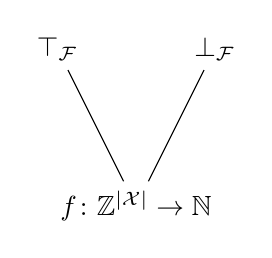
\begin{tikzpicture}[]
            \node (top) at (0,2) {$\top_{\mathcal{F}}$};
            \node (bot) at (2,2) {$\bot_{\mathcal{F}}$};
            \node (f) at (1,0) {$f \colon  \mathbb{Z}^{|\mathcal{X}|} \rightarrow \mathbb{N} $};
            \draw (top) -- (f) -- (bot);
        \end{tikzpicture}
        \caption{\textit{approximation order} $\preceq_{\mathcal{F}}$}
    \end{subfigure}
    \caption{Hasse diagrams for $\sqsubseteq_{\mathcal{F}}$ and $\preceq_{\mathcal{F}}$
    } 
    \label{fig:function_comp_approx_hasse}
\end{figure}

\subsection{Join}\label{sec:tree_join}
Two trees can be joined to form the union of all partitions represented by the two trees. When joining two trees, they are first reshaped such
that both trees consist of the same partitions. They only differ in the values of the leafs. Then the two trees can be joined leaf-wise. 
There are two join variations. 
The \textit{computational join} $\sqcup_{\mathcal{T}} \colon (\mathcal{T}_{NIL} \times \mathcal{T}_{NIL}) \rightarrow \mathcal{T}_{NIL}$
and the \textit{approximation join} $\curlyvee_{\mathcal{T}} \colon (\mathcal{T}_{NIL} \times \mathcal{T}_{NIL}) \rightarrow \mathcal{T}_{NIL}$. 
Two leafs $l_1$ and $l_2$ are joined by taking the least upper bound of the two functions $l_1.f$ and $l_2.f$ 
w.r.t. $\sqsubseteq_{\mathcal{F}}$ ($\preceq_{\mathcal{F}}$, respectively).
Figure~\ref{fig:decision_tree_join_example} demonstrates the difference between the two join types. 
When joining two trees where one leaf is defined and one is undefined 
(see left leaf in $t_1$ and $t_2$), the \textit{computational join} will preserve the defined leaf
and the \textit{approximation join} will make the leaf undefined. If one of the two leafs is $\mathtt{NIL}$ then they are joined by taking the one
that is not $\mathtt{NIL}$. When both are $\mathtt{NIL}$ then the result of joining the leafs is $\mathtt{NIL}$.

\begin{figure}
    \begin{subfigure}[b]{0.5\textwidth}
        \centering
        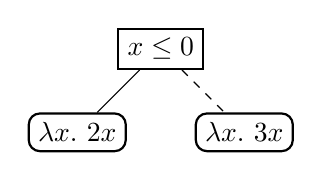
\begin{tikzpicture}[node distance=1.5cm]
            \tikzset{
                inner_node/.style={draw, shape = rectangle, thick},
                leaf/.style={draw, shape = rectangle, rounded corners, thick}
            }
            \node[inner_node] (A) {$x \leq 0$};
            \node[leaf] (B) [below left of= A] {$\lambda x.\ 2x$};
            \node[leaf] (C) [below right of= A] {$\lambda x. \ 3x$};

            \path (A) edge              node {} (B);
            \path (A) edge [dashed]              node {} (C);
        \end{tikzpicture}
        \caption{$t_1$}
    \end{subfigure}
    \begin{subfigure}[b]{0.5\textwidth}
        \centering
        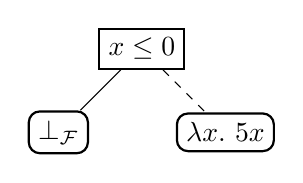
\begin{tikzpicture}[node distance=1.5cm]
            \tikzset{
                inner_node/.style={draw, shape = rectangle, thick},
                leaf/.style={draw, shape = rectangle, rounded corners, thick}
            }
            \node[inner_node] (A) {$x \leq 0$};
            \node[leaf] (B) [below left of= A] {$\bot_{\mathcal{F}}$};
            \node[leaf] (C) [below right of= A] {$\lambda x. \ 5x$};
            \path (A) edge              node {} (B);
            \path (A) edge [dashed]              node {} (C);
        \end{tikzpicture}
        \caption{$t_2$}
    \end{subfigure}
    \par\bigskip
    \begin{subfigure}[b]{0.5\textwidth}
        \centering
        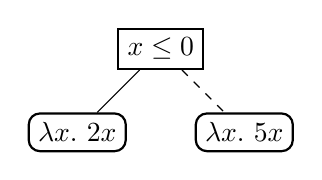
\begin{tikzpicture}[node distance=1.5cm]
            \tikzset{
                inner_node/.style={draw, shape = rectangle, thick},
                leaf/.style={draw, shape = rectangle, rounded corners, thick}
            }
            \node[inner_node] (A) {$x \leq 0$};
            \node[leaf] (B) [below left of= A] {$\lambda x.\ 2x$};
            \node[leaf] (C) [below right of= A] {$\lambda x. \ 5x$};
            \path (A) edge              node {} (B);
            \path (A) edge [dashed]              node {} (C);
        \end{tikzpicture}
        \caption{$t_1 \sqcup_{\mathcal{T}} t_2$}
    \end{subfigure}
    \begin{subfigure}[b]{0.5\textwidth}
        \centering
        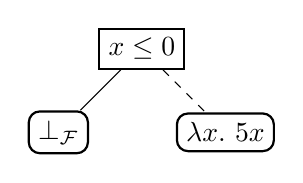
\begin{tikzpicture}[node distance=1.5cm]
            \tikzset{
                inner_node/.style={draw, shape = rectangle, thick},
                leaf/.style={draw, shape = rectangle, rounded corners, thick}
            }
            \node[inner_node] (A) {$x \leq 0$};
            \node[leaf] (B) [below left of= A] {$\bot_{\mathcal{F}}$};
            \node[leaf] (C) [below right of= A] {$\lambda x. \ 5x$};

            \path (A) edge              node {} (B);
            \path (A) edge [dashed]              node {} (C);
        \end{tikzpicture}
        \caption{$t_1 \curlyvee_{\mathcal{T}} t_2$}
    \end{subfigure}

    \caption{Decision Tree Join Example}
    \label{fig:decision_tree_join_example}
\end{figure}


\subsection{Meet}\label{sec:tree_meet}
The meet operator intersects the partitions of two decision trees. As with the join, both trees are first
brought into the same shape such that they can be combined leaf-wise. There are two meet variations. 
The \textit{computational meet} $\sqcap_\mathcal{T} \colon (\mathcal{T}_\mathtt{NIL} \times \mathcal{T}_\mathtt{NIL}) \rightarrow \mathcal{T}_\mathtt{NIL}$
and the \textit{approximation meet} $\curlywedge_\mathcal{T} \colon (\mathcal{T}_\mathtt{NIL} \times \mathcal{T}_\mathtt{NIL}) \rightarrow \mathcal{T}_\mathtt{NIL}$. 
Both combine defined leafs using the least upper bound w.r.t.\ $\preceq_{\mathcal{F}}$. 
If at least one of the two leafs is \texttt{NIL}, then the result is $\bot_\mathcal{F}$ in case of the 
\textit{computational meet} and \texttt{NIL} in case of the \textit{approximation meet}.

\subsection{Widening and Dual Widening}\label{sec:tree_widen}
The \textit{widening} operator $\triangledown_\mathcal{T} \colon (\mathcal{T}_\mathtt{NIL} \times \mathcal{T}_\mathtt{NIL}) \rightarrow \mathcal{T}_\mathtt{NIL}$
is used to enforce convergence when computing increasing sequences of values in the decision tree abstract domain. 
Once the sequence is stable for the \textit{computational order} $\sqsubseteq_\mathcal{T}$, 
the limit of this sequence is guaranteed to be a sound approximation of the corresponding concrete counting function 
w.r.t.\ the \textit{approximation order} $\preceq_{\mathcal{F}}$.
The dual of this concept for decreasing sequences is called \textit{dual widening} 
$\bar\triangledown_\mathcal{T} \colon (\mathcal{T}_\mathtt{NIL} \times \mathcal{T}_\mathtt{NIL}) \rightarrow \mathcal{T}_\mathtt{NIL}$.
Intuitively, the widening operator tries to extrapolate the function values of decision trees to linear functions. This extrapolation is
initially a guess. If the guess proves to be wrong, it is corrected by setting the corresponding partition to $\top_\mathcal{T}$ in future iterations.
A thorough discussion about widening for elements of the decision tree abstract domain can be found in Section 5.2.4 of~\cite{UrbanPhd}.


\subsection{Filter}\label{sec:tree_filter}
The filter operator $\mathtt{FILTER}_o\llbracket bexp \rrbracket \colon \mathcal{T}_\mathtt{NIL} \rightarrow \mathcal{T}_\mathtt{NIL}$
prunes all partitions of a decision tree that do not satisfy the given boolean expression $bexp$. Leafs are pruned by replacing them with \texttt{NIL}.
Partitions are pruned using over-approximation.
That means that the resulting tree can still be defined for states that do not satisfy the boolean expression. It is however guaranteed that all states 
that satisfy the boolean expression remain defined in the tree. In addition to the over-approximating version there is also the under-approximating version
$\mathtt{FILTER}_u \llbracket bexp \rrbracket \colon \mathcal{T}_\mathtt{NIL} \rightarrow \mathcal{T}_\mathtt{NIL}$. Here the resulting decision
tree is guaranteed to not contain any partitions that do not satisfy the boolean expressions. However states that do satisfy it might be removed if
the underlying numerical domain is not expressive enough.

\subsection{Backward Assign}\label{sec:tree_bwd_assign}
The operator $\mathtt{ASSIGN}_o \llbracket X := \mathtt{aexp} \rrbracket \colon \mathcal{T}_\mathtt{NIL} \rightarrow \mathcal{T}_\mathtt{NIL}$ handles
the backward assignment of the arithmetic expression \texttt{aexp} to variable $X$. The linear constraints of the decision tree nodes and the 
functions at the leafs are adjusted accordingly. $\mathtt{ASSIGN}_o$ uses over-approximation on the underlying numerical domains. 
As with the filter operator, there also exists an under-approximating version 
$\mathtt{ASSIGN}_u \llbracket X := \mathtt{aexp} \rrbracket \colon \mathcal{T}_\mathtt{NIL} \rightarrow \mathcal{T}_\mathtt{NIL}$.


\section{Abstract Semantics for CTL}\label{sec:abstract_ctl_semantics}

The counting function $\tau_\Phi$ is in general not computable. 
In this section we present a sound and computable approximation of the \textit{CTL semantics} $\tau_\Phi$ defined in Section~\ref{sec:ctl_semantics}.
We approximate $\tau_\Phi$ by using the decision tree abstract domain (Section~\ref{sec:decision_tree_abstract_domain}) 
to approximate counting functions in terms of piecewise defined ranking functions.

\begin{theorem}\label{thr:abstract_ctl_semantics}
    The abstract CTL semantics $\tau^{\sharp}_\Phi \in \mathcal{L} \rightarrow \mathcal{T}$ is a sound approximation of the
    CTL semantics $\tau_\Phi$ with regards to the \textit{approximation order} $\preceq_\mathcal{T}$ (see Definition~\ref{def:sound_abstraction}).
\end{theorem}

Recall that the CTL semantics $\tau_\Phi \in \Sigma \rightarrow \mathbb{N}$ is a partial function that 
assigns numerical values to program states $\sigma \in \Sigma$. 
In the abstract version, program states are grouped by program labels $l \in \mathcal{L}$ and
partitioned by decision trees $t \in \mathcal{T}$. 
A program satisfies a given CTL property $\Phi$ if the decision tree of the
initial program label $\tau^{\sharp}_\Phi(t_{init})$ is defined over all partitions of program states, i.e., 
all leafs of the decision tree are defined.\\

The following sections present how to compute $\tau^{\sharp}_\Phi$ for each CTL operator. 
We start with the basic operators $\land, \lor, \neg$ and atomic propositions. 
These can be computed directly for each program label. 
Then we present how to compute the universal $\forall(\cdot U \cdot)$, $\forall\bigcirc$ and $\forall\square$ operators through fixed-point iteration. 
Followed by a discussion on how to adapt the universal operators to their existential version. 
Note that the abstract CTL semantics are computed recursively. The recursion stops at atomic propositions.

\subsection{Path Independent Operators}

Atomic propositions are path independent, therefore $\tau^{\sharp}_a$ assigns the same decision tree to 
each program label $l \in \mathcal{L}$. This decision tree assigns the constant function $0$ to all partitions that satisfy the atomic proposition $a$.
We compute this tree by using the $\mathtt{RESET} \llbracket a \rrbracket$ operator on the totally undefined decision tree $\bot_\mathcal{T}$. 
The $\mathtt{RESET}\llbracket a \rrbracket \colon \mathcal{T} \rightarrow \mathcal{T}$ operator takes as input a decision tree and returns a copy of 
said tree where every partition that satisfies $a$ is replaced with the constant function $0$. We refer the reader to~\cite{UrbanPhd}
for a detailed description of the $\mathtt{RESET}$ operator. Note however, that the implementation of $\mathtt{RESET}$ in~\cite{UrbanPhd} 
has a small error that can lead to unsoundness. This is discussed in the excursion below titled `$\mathtt{RESET}$ and over-approximation'.


\begin{definition}\label{def:abstract_ctl_semantics_atomic}
    Abstract CTL semantics for atomic propositions
    \begin{align}
        \tau^{\sharp}_{a} \eqdef \ \lambda l. \ \mathtt{RESET} \llbracket a \rrbracket \bot_\mathcal{T}
    \end{align}
\end{definition}

\begin{lemma}
    The abstract CTL semantics $\tau^{\sharp}_{a}$ is a sound approximation of the
    CTL semantics $\tau_{a}$ with regards to the \textit{approximation order} $\preceq_\mathcal{T}$ (see Definition~\ref{def:sound_abstraction}).
\end{lemma}


\begin{tcolorbox}
    \subsubsection*{$\mathtt{RESET}$ and over-approximation}

    The $\mathtt{RESET}\llbracket a \rrbracket$ operator was originally introduced in~\cite{UrbanPhd} in the context of abstract guarantee semantics
    and would over-approximate the set of partitions that satisfy the atomic proposition $a$. 
    During the work on this thesis, we discovered that this original definition is actually unsound and leads to incorrect analysis results.\\
    
    The problem is best described using an example. Consider the abstract CTL semantics $\tau^{\sharp}_{x^2 < y^3 + 1}$. 
    The non-linear constraint $x^2 < y^3 + 1$ can usually not be represented by any of the commonly used numerical domains. 
    An over-approximating implementation of $\mathtt{RESET}\llbracket x^2 < y^3 + 1 \rrbracket$ will therefore
    reset some pairs $(x, y)$ for which $x^2 < y^3 + 1$ does not hold which is unsound as to the definition of
    the CTL semantics $\tau_{x^2 < y^3 + 1}$. Note that this problem propagates to more complex temporal properties that
    depend on atomic propositions.\\

    We resolve this problem by using under-approximating on the underlying numerical domains to soundly determine which partitions 
    satisfy the atomic proposition $a$. 
\end{tcolorbox}

Now we define the abstract CTL semantics for the logical operators $\land$, $\lor$ and $\neg$.

\begin{definition}\label{def:abstract_ctl_semantics_logic_operators}
    Abstract CTL semantics for logic operators
    \begin{align}
        \tau^{\sharp}_{\Phi_1 \land \Phi_2} &\eqdef \ \lambda l. \ (\tau^{\sharp}_{\neg \Phi_1}l) \ \sqcup_{\mathcal{T}} \ (\tau^{\sharp}_{\neg \Phi_2}l)
        \label{eq:abstract_ctl_and}\\
        \tau^{\sharp}_{\Phi_1 \lor \Phi_2} &\eqdef \ \lambda l. \ (\tau^{\sharp}_{\neg \Phi_1}l) \ \sqcap_{\mathcal{T}} \ (\tau^{\sharp}_{\neg \Phi_2}l)
        \label{eq:abstract_ctl_or}\\
        \tau^{\sharp}_{\neg \Phi} &\eqdef \ \lambda l. \ \mathtt{COMPLEMENT} \ (\tau^{\sharp}_{\neg \Phi}l)
        \label{eq:abstract_ctl_not}
    \end{align}
\end{definition}

The abstract CTL semantics for $\land$ and $\lor$ (Equations~\ref{eq:abstract_ctl_and} and~\ref{eq:abstract_ctl_or}) combine the decision trees
of the nested properties piecewise for each program label.\\

The \textit{computational join} $\sqcup_{\mathcal{T}}$ is used to combine the two trees (see Section~\ref{sec:tree_join}) in
case of the logical $\lor$. This operator forms the union of the two decision trees. 
Note that we use the computational version of the join operator to include partitions that are defined in at least one of the two trees. 
If a partition is defined in both trees, the least upper bound of the two functions assigned to that partition is used w.r.t.\ to the 
partial order $\sqsubseteq_{\mathcal{F}}$ given in Definition~\ref{def:fun_comp_approx_order}.\\

The corresponding definition for the logical $\land$ operator forms the intersection of the two trees by using the
\textit{computational meet} $\sqcap_{\mathcal{T}}$ (see Section~\ref{sec:tree_meet}). 
By using the computational version of the meet, we ensure that no $\mathtt{NIL}$ leafs are introduced when forming the intersection.
As with the logical $\lor$, the least upper bound w.r.t.\ to $\sqsubseteq_{\mathcal{F}}$ is used if a partition is defined in both trees.\\

For the logical $\neg$ operator we introduce the $\mathtt{COMPLEMENT}\colon \mathcal{T}_\mathtt{NIL} \rightarrow \mathcal{T}_\mathtt{NIL}$ operator. 
This operator replaces all defined leafs with a $\bot$-leaf and all $\bot$-leafs with the constant function $0$.
By doing so, all states that originally satisfied the property do not satisfy it any more and vice versa.
However one has to be careful when changing a partition from undefined to defined. Decision trees are an 
approximation of the concrete CTL semantics. Therefore not all states that are undefined in the abstract decision tree
are actually undefined in the concrete ranking function. Partitions that are undefined because of this uncertainty are marked with a 
$\top$-leaf. To ensure soundness, these leafs have to be ignored when forming the complement of a decision tree.   
The $\mathtt{COMPLEMENT}$ operator is implemented in Algorithm~\ref{alg:tree_complement}.


\begin{lemma}
    The abstract CTL semantics $\tau^{\sharp}_{\Phi_1 \land \Phi_2}$, $\tau^{\sharp}_{\Phi_1 \lor \Phi_2}$ and $\tau^{\sharp}_{\neg \Phi}$ 
    are a sound approximation of the CTL semantics
    $\tau_{\Phi_1 \land \Phi_2}$, $\tau_{\Phi_1 \lor \Phi_2}$ and $\tau_{\neg \Phi}$ with regards to the 
    \textit{approximation order} $\preceq_\mathcal{T}$ (see Definition~\ref{def:sound_abstraction}).
\end{lemma}


\begin{algorithm}[t]                    
    \caption{Tree Complement}         
    \label{alg:tree_complement}       
    \begin{algorithmic}
        \Function{complement}{$t$} 
        \Comment{$t \in \mathcal{T}_{NIL}$}
        \If{$(isNode(t) \land t.f = \top) \lor isNil(t)$}
            \State \Return $t$
            \Comment{ignore $\top$ and $NIL$}
        \ElsIf{$isLeaf(t) \land t.f = \bot$}
            \State \Return $LEAF: 0$
            \Comment{undefined becomes defined}
        \ElsIf{$isLeaf(t)$}
            \State \Return $LEAF: \bot$
            \Comment{defined becomes undefined}
        \Else
            \State $l \gets \Call{complement}{t.l}$
            \State $r \gets \Call{complement}{t.r}$
            \State \Return $NODE\{t.c \}: l ; r$
        \EndIf
        \EndFunction
\end{algorithmic}
\end{algorithm}


\subsection{Path Dependent Operators}

In this section we describe how the abstract CTL semantics for the path-dependent operators 
($\forall\bigcirc\Phi,\ \exists\bigcirc\Phi,\ \forall(\Phi_1 U \Phi_2),\ \exists(\Phi_1 U \Phi_2),\ \forall\square\Phi,\ \exists\square\Phi$)
are defined.\\

First, we define the two functions ${\llbracket stmt \rrbracket}_o \in \mathcal{T}_{NIL} \rightarrow \mathcal{T}_{NIL}$
and ${\llbracket stmt \rrbracket}_u \in \mathcal{T}_{NIL} \rightarrow \mathcal{T}_{NIL}$. 
The first one uses over-approximation on the underlying numerical domains, the second one under-approximation.\\

Both functions implement the effect of backward propagating an edge 
in the control-flow-graph, i.e., the effect of executing a statement. 
Assume that we have computed a decision tree for the target node of some edge. 
This decision tree represents the value of the counting function for this node. 
By applying ${\llbracket \cdot \rrbracket}$ to this tree, we compute the decision tree 
that holds before executing the statement, i.e.\, the value of the function at the source node of this edge.



\begin{definition}\label{def:basic_expression_transformer}
    Abstract semantics for basic statements
    \begin{align*}
        {\llbracket \mathtt{skip} \rrbracket}_o \eqdef \lambda t. \ \mathtt{STEP}(t)\\
        {\llbracket bexp \rrbracket}_o \eqdef \lambda t. \ \mathtt{ASSIGN}_o(t)\\
        {\llbracket X := aexp \rrbracket}_o \eqdef \lambda t. \ \mathtt{FILTER}_o(t)\\
        \\
        {\llbracket \mathtt{skip} \rrbracket}_u \eqdef \lambda t. \ \mathtt{STEP}(t)\\
        {\llbracket bexp \rrbracket}_u \eqdef \lambda t. \ \mathtt{ASSIGN}_u(t)\\
        {\llbracket X := aexp \rrbracket}_u \eqdef \lambda t. \ \mathtt{FILTER}_u(t)\\
    \end{align*}
\end{definition}

The \texttt{skip} statement is handled by the $\mathtt{STEP}$ operator. This operator increases the value of all defined
partitions in the decision tree by one. Recall that a defined partition in a decision tree represents a set of states that satisfies 
some CTL property. The associated value is an upper bound on the number of steps until some condition is reached. 
By executing \texttt{skip} this number is incremented by one.
For assignments and boolean conditions we use the corresponding \textit{assign} and \textit{filter}
operators that were introduced in Sections~\ref{sec:tree_bwd_assign} and~\ref{sec:tree_filter}.
The definitions for the remaining path dependent operators all depend on these two functions.

\subsubsection*{Until}
The abstract CTL semantics for universal and existential \textsf{until} properties are defined as the least fixed-point of the abstract transformers

\begin{align*}
    \phi^\sharp_{\forall(\Phi_1 U \Phi_2)}
    \in (\mathcal{L} \rightarrow \mathcal{T}_{NIL}) \rightarrow (\mathcal{L} \rightarrow \mathcal{T}_{NIL})\\
    \phi^\sharp_{\exists(\Phi_1 U \Phi_2)} 
    \in (\mathcal{L} \rightarrow \mathcal{T}_{NIL}) \rightarrow (\mathcal{L} \rightarrow \mathcal{T}_{NIL})
\end{align*}
starting from the function $\tau_\bot$ that assigns the decision tree $\bot_\mathcal{T}$ to every 
node in the control-flow-graph. $\forall l \in \mathcal{L} \colon \tau_\bot(l) = \bot_\mathcal{T}$.

\begin{definition}\label{def:abstract_until_semantics}
    Abstract semantics for \textsf{until} operator. 
    \setlength{\jot}{15pt}
    \begin{align*}
        \tau^\sharp_{\forall(\Phi_1 U \Phi_2)} \ &\eqdef \ \text{lfp}^{\sqsubseteq_{\mathcal{T}}}_{\tau_\bot} \phi^\sharp_{\forall(\Phi_1 U \Phi_2)}\\
        t_{\curlyvee}(m, l)  \ &\eqdef \ \bigcurlyvee\limits_{(l, stmt, l') \ \in \ out(l) } {\llbracket stmt \rrbracket}_{o} ( m(l')) \\
        \phi^\sharp_{\forall(\Phi_1 U \Phi_2)}(m)l \ &\eqdef \ \mathtt{UNTIL}\llbracket \tau^\sharp_{\Phi_1}(l), \tau^\sharp_{\Phi_2}(l) \rrbracket (t_{\curlyvee}(m, l))  \\\\
        %
        %
        \tau^\sharp_{\exists(\Phi_1 U \Phi_2)} \ &\eqdef \ \text{lfp}^{\sqsubseteq_{\mathcal{T}}}_{\bot_\mathcal{T}} \phi^\sharp_{\exists(\Phi_1 U \Phi_2)}\\
        t_{\sqcup}(m, l) \ &\eqdef \ \bigsqcup\limits_{(l, stmt, l') \ \in \ out(l) } {\llbracket stmt \rrbracket}_{u} (m(l')) \\
        \phi^\sharp_{\exists(\Phi_1 U \Phi_2)}(m)l \ &\eqdef \ \mathtt{UNTIL}\llbracket \tau^\sharp_{\Phi_1}(l), \tau^\sharp_{\Phi_2}(l) \rrbracket ( t_{\sqcup}(m, l))
    \end{align*}\\
\end{definition}

We will first discuss the universal version and then explain what changes for the existential case.
The value $m \in \mathcal{L} \rightarrow \mathcal{T}_{NIL}$ is the current iteration value of the fixed-point iteration, 
$\phi^\sharp_{\forall(\Phi_1 U \Phi_2)}(m)$ describes the value of the next iteration.
Recall that $out(l)$ denotes all outgoing edges of node $l$ leading to its immediate successors nodes. Every edge is labeled with a statement. 
The abstract transformer $\phi^\sharp_{\forall(\Phi_1 U \Phi_2)}$ computes decision trees point-wise for each node $l$ in the 
control-flow-graph, based on the decision trees of its successor nodes.\\

First, the decision tree of each successor node $l'$ is passed to the ${\llbracket stmt \rrbracket}_{o}$ function. 
This approximates the effect of transitioning from $l$ to $l'$. The resulting decision tree approximates the value of 
the ranking function before executing the statement.\\

If a node has multiple successor nodes then the resulting decision trees 
are combined using the \textit{approximation join} $\curlyvee$. 
The \textit{approximation join} discards all partitions (i.e., makes them undefined)
of decision trees that are not defined for all successor nodes. By doing so, we approximate the semantic of the universal path  
quantifier $\forall$. Note that if a node has no successors then $t_{\curlyvee}(m, l) = \bot_{\mathcal{T}}$ since
the least upper bound (join) of the empty set is $\bot_\mathcal{T}$.\\

We use the over-approximating version of the ${\llbracket \cdot \rrbracket}_{o}$ function. 
This might temporarily lead to unsound decision trees due to over-approximation. 
Decision trees produced by ${\llbracket \cdot \rrbracket}_{o}$ can contain defined partitions for states that are unfeasible 
among that path in the control-flow-graph. For the universal case however, this is not a problem since the 
\textit{approximation join} only keeps those partitions which are feasible among all paths. 
Partitions that are unfeasible among some paths are discarded.\\

Finally the result of joining the decision trees of the immediate predecessors are 
applied to he $\mathtt{UNTIL}\llbracket \tau^\sharp_{\Phi_1}, \tau^\sharp_{\Phi_2} \rrbracket $ operator. 
The purpose of his operator is to implement the semantics of the \textsf{until} CTL operator. 
All partitions that satisfy $\Phi_1$ are set to zero and all partitions that neither 
satisfy $\Phi_1$ nor $\Phi_2$ are discarded (see Algorithm~\ref{alg:tree_until}).
That way we end up with a decision tree that is only defined for the partitions that satisfy $\forall(\Phi_1 U \Phi_2)$.\\

The abstract transformer for the existential case follows the same structure as in the universal case. 
However instead of using the \textit{approximation join} it uses the \textit{computational join} $\sqcup_\mathcal{T}$ 
to approximate the semantics of the $\exists$ path quantifier. 
The \textit{computational join} preserves all partitions that are defined for at least one decision tree. 
Note however, that all decision trees passed to the \textit{computation join} must be sound since we can no longer 
rely on the join operator to discard unfeasible partitions. Therefore we apply the under-approximating ${\llbracket stmt \rrbracket}_{u}$ 
function when processing statements to guarantee soundness.\\

\begin{lemma}
    The abstract CTL semantics 
    $\tau^{\sharp}_{\forall(\Phi_1 U \Phi_2)}$ and $\tau^{\sharp}_{\exists(\Phi_1 U \Phi_2)}$
    are a sound approximation of the CTL semantics
    $\tau_{\forall(\Phi_1 U \Phi_2)}$ and $\tau_{\exists(\Phi_1 U \Phi_2)}$
    with regards to the \textit{approximation order} $\preceq_\mathcal{T}$ (see Definition~\ref{def:sound_abstraction}).\\
\end{lemma}

Convergence of the least fixed-point iteration is guaranteed after a finite amount of iterations by using the widening operator $\triangledown_\mathcal{T}$ 
(see Section~\ref{sec:tree_widen}). The decision tree computed for every node $l \in \mathcal{L}$ is guaranteed to converge by applying the following widening scheme 
($\Phi_U$ is a placeholder for $\forall(\Phi_1 U \Phi_2)$ and $\exists(\Phi_1 U \Phi_2)$):

\begin{align*}
    y_0 &\eqdef \bot_\mathcal{T}\\
    y_{n+1} &\eqdef 
    \begin{cases}
        y_n                   &\text{if} \ \phi^\sharp_{\Phi_{U}}(y_n) \sqsubseteq_\mathcal{T} y_n 
        \land \phi^\sharp_{\Phi_U}(y_n) \preceq_\mathcal{T} y_n  \\
        y_n \ \triangledown_\mathcal{T} \ \phi^\sharp_{\Phi_U}(y_n)     &\text{otherwise}
    \end{cases}
\end{align*}

\begin{algorithm}[t]
    \caption{Tree Until Filter}         
    \label{alg:tree_until_filter}       
    \begin{algorithmic}
        \Function{filter\_until}{$t, t_{\text{valid}}$} 
            \If{$isNil(t) \lor isNil(t_{\text{valid}})$}
                \LineComment{ignore $NIL$ nodes}
                \State \Return $t$
            \ElsIf{$isLeaf(t) \land isLeaf(t_{\text{valid}}) \land isDefined(t)$}
                \LineComment{$t$ is defined in $t_{\text{valid}}$}
                \State \Return $t$
            \ElsIf{$isLeaf(t) \land isLeaf(t_{\text{valid}}) \land  \neg isDefined(t)$}
                \LineComment{$t$ is not defined in $t_{\text{valid}}$, make undefined}
                \State \Return $LEAF: \bot$
            \Else
                \State $l \gets \Call{filter\_until}{t.l, t_{\text{valid}}.l}$
                \State $r \gets \Call{filter\_until}{t.r, t_{\text{valid}}.r}$
                \State \Return $NODE\{t.c \}: l ; r$
            \EndIf 
        \EndFunction
\end{algorithmic}
\end{algorithm}

\begin{algorithm}[t]                    
    \caption{Tree Until}         
    \label{alg:tree_until}       
    \begin{algorithmic}
        \Function{reset\_until}{$t, t_{\text{reset}}$} 
            \If{$isNil(t) \lor isNil(t_{\text{reset}})$}
                \LineComment{ignore $NIL$ nodes}
                \State \Return $t$
            \ElsIf{$isLeaf(t) \land isLeaf(t_{\text{reset}}) \land isDefined(t)$}
                \LineComment{$t$ is defined in $t_{\text{valid}}$, reset leaf}
                \State \Return $LEAF: 0$
            \ElsIf{$isLeaf(t) \land isLeaf(t_{\text{valid}}) \land  \neg isDefined(t)$}
                \LineComment{$t$ is undefined in $t_{\text{valid}}$, keep as is}
                \State \Return $t$
            \Else
                \State $l \gets \Call{reset\_until}{t.l, t_{\text{reset}}.l}$
                \State $r \gets \Call{reset\_until}{t.r, t_{\text{reset}}.r}$
                \State \Return $NODE\{t.c \}: l ; r$
            \EndIf 
        \EndFunction
        \Function{until$\llbracket t_{\Phi_1}, t_{\Phi_2} \rrbracket$}{$t$} 
            \Comment{$t, t_{\Phi_1}, t_{\Phi_2} \in \mathcal{T}_{NIL}$}
            \State $(t_1, t_2) \gets \Call{tree\_unification}{t, t_{\Phi_1} \sqcup t_{\Phi_2}}$
            \State $t_{\text{filtered}} \gets \Call{filter\_until}{t_1, t_2}$
            \State $(t_1, t_2) \gets \Call{tree\_unification}{t_{\text{filtered}}, t_{\Phi_2}}$
            \State \Return $\Call{reset\_until}{t_1, t_2}$
        \EndFunction
\end{algorithmic}
\end{algorithm}




\subsubsection*{Global}
The abstract CTL semantics for universal and existential \textsf{global} properties are defined as the greatest fixed-point of the abstract transformers

\begin{align*}
    \phi^\sharp_{\forall\square\Phi} \in (\mathcal{L} \rightarrow \mathcal{T}_{NIL}) \rightarrow (\mathcal{L} \rightarrow \mathcal{T}_{NIL})\\
    \phi^\sharp_{\exists\square\Phi} \in (\mathcal{L} \rightarrow \mathcal{T}_{NIL}) \rightarrow (\mathcal{L} \rightarrow \mathcal{T}_{NIL})
\end{align*}
starting from the abstract CTL semantics $\tau^\sharp_\Phi$ of the inner CTL property $\Phi$.

\begin{definition}\label{def:abstract_global_semantics}
    Abstract semantics for \textsf{global} operator.
    \setlength{\jot}{15pt}
    \begin{align*}
        \tau^\sharp_{\forall\square\Phi} \ &\eqdef \ \text{gfp}^{\sqsubseteq_{\mathcal{T}}}_{\tau^\sharp_\Phi} \phi^\sharp_{\forall\square\Phi}\\
        t_{\curlyvee}(m, l)  \ &\eqdef \ \bigcurlyvee\limits_{(l, stmt, l') \ \in \ out(l) } {\llbracket stmt \rrbracket}_{o} ( m(l')) \\
        \phi^\sharp_{\forall\square\Phi}(m)l \ &\eqdef \ \mathtt{MASK}\llbracket t_{\curlyvee}(l,m)\rrbracket (m(l))  \\\\
        %
        \tau^\sharp_{\exists\square\Phi} \ &\eqdef \ \text{gfp}^{\sqsubseteq_{\mathcal{T}}}_{\tau^\sharp_\Phi} \phi^\sharp_{\exists\square\Phi}\\
        t_{\sqcup}(m, l)  \ &\eqdef \ \bigsqcup\limits_{(l, stmt, l') \ \in \ out(l) } {\llbracket stmt \rrbracket}_{u} ( m(l')) \\
        \phi^\sharp_{\exists\square\Phi}(m)l \ &\eqdef \ \mathtt{MASK}\llbracket t_{\sqcup}(l,m) \rrbracket (m(l))  \\\\
    \end{align*}
\end{definition}

The value $m \in \mathcal{L} \rightarrow \mathcal{T}_{NIL}$ is the current iteration value of the fixed-point iteration. 
The definition for $\phi^\sharp_{\forall\square\Phi}(m)$ ($\phi^\sharp_{\exists\square\Phi}(m)$, respectively) describes the value of the next iteration.
We use the same approach as the \textsf{until} operator to join decision trees of successor nodes
(see $t_{\curlyvee}(m, l)$ and $t_{\sqcup}(m, l)$).\\

In the final step however, the decision tree $m(l)$ of each node $l$ is \textit{masked} with the result of $t_{\curlyvee}(l,m)$ ($t_{\sqcup}(l,m)$ respectively).
Masking is implemented by the \texttt{MASK} operator. This operator sets all partitions of $m(l)$ to $\bot_\mathcal{T}$,
that are not defined in $t_{\curlyvee}(l,m)$ ($t_{\sqcup}(l,m)$, respectively).
That way all states that do not satisfy $\Phi$ indefinitely among all (some, respectively) paths are iteratively 
removed from the decision tree until a fixed-point is reached. 
The \texttt{MASK} operator is defined in Algorithm~\ref{alg:tree_mask}.


\begin{lemma}
    The abstract CTL semantics 
    $\tau^{\sharp}_{\forall\square\Phi}$ and $\tau^{\sharp}_{\exists\square\Phi}$
    are a sound approximation of the CTL semantics
    $\tau_{\forall\square\Phi}$ and $\tau_{\exists\square\Phi}$
    with regards to the \textit{approximation order} $\preceq_\mathcal{T}$ (see Definition~\ref{def:sound_abstraction}).\\
\end{lemma}

Convergence of the greatest fixed-point iteration is guaranteed after a finite amount of iterations by using the dual 
widening operator $\bar\triangledown_\mathcal{T}$  (see Section~\ref{sec:tree_widen}). 
The decision tree computed for every node $l \in \mathcal{L}$ is guaranteed to converge by applying the following widening scheme 
($\Phi_G$ is a placeholder for $\forall\square\Phi$ and $\exists\square\Phi$):

\begin{align*}
    y_0 &\eqdef \tau^\sharp_{\Phi_U}(l)\\
    y_{n+1} &\eqdef 
    \begin{cases}
        y_n                   &\text{if} \ y_n \sqsubseteq_\mathcal{T} \phi^\sharp_{\Phi_{G}}(y_n)  
        \land y_n \preceq_\mathcal{T} \phi^\sharp_{\Phi_G}(y_n)  \\
        y_n \ \bar\triangledown_\mathcal{T} \ \phi^\sharp_{\Phi_G}(y_n)     &\text{otherwise}
    \end{cases}
\end{align*}


\begin{algorithm}[t]
    \caption{Tree Mask}         
    \label{alg:tree_mask}       
    \begin{algorithmic}
        \Function{mask$\llbracket t_{\text{mask}} \rrbracket$}{$t$} 

            \Function{mask\_aux}{$t, t_{\text{mask}} $} 
                \If{$isNil(t) \lor isNil(t_{\text{reset}})$}
                    \LineComment{ignore $NIL$ nodes}
                    \State \Return $t$
                \ElsIf{$isLeaf(t) \land isDefined(t) \land isLeaf(t_{\text{mask}})$}
                    \If{$isDefined(t) \land \neg isDefined(t_{\text{mask}})$}
                        \LineComment{$t$ is defined and $t_{\text{mask}}$ is undefined, discard leaf}
                        \State \Return $LEAF: \bot$
                    \Else
                        \State \Return $t$
                    \EndIf
                \Else
                    \State $l \gets \Call{mask}{t.l, t_{\text{mask}}.l}$
                    \State $r \gets \Call{mask}{t.r, t_{\text{mask}}.r}$
                    \State \Return $NODE\{t.c \}: l ; r$
                \EndIf 
            \EndFunction

            \State $(t_1, t_2) \gets \Call{tree\_unification}{t, t_{\text{MASK}}}$
            \State \Return $\Call{mask\_aux}{t_1, t_2}$
        \EndFunction
\end{algorithmic}
\end{algorithm}



\subsubsection*{Next}
The abstract CTL semantics for the \textsf{next} operator are given in Definition~\ref{def:abstract_next_semantics}: 

\begin{definition}\label{def:abstract_next_semantics}
    Abstract semantics for \textsf{next} operator.
    \setlength{\jot}{15pt}
    \begin{align*}
        t_{\curlyvee}(l) \ &\eqdef \  
        \bigcurlyvee\limits_{(l, stmt, l') \ \in \ out(l) } {\llbracket stmt \rrbracket}_{o}(\tau^\sharp_\Phi(l)) \\
        \tau^\sharp_{\forall\bigcirc\Phi} \ &\eqdef \ \lambda l. \ \mathtt{ZERO}(t_{\curlyvee}(l))\\\\
        %
        t_{\sqcup}(l) \ &\eqdef \  
        \bigsqcup\limits_{(l, stmt, l') \ \in \ out(l) } {\llbracket stmt \rrbracket}_{u}(\tau^\sharp_\Phi(l)) \\
        \tau^\sharp_{\exists\bigcirc\Phi} \ &\eqdef \ \lambda l. \ \mathtt{ZERO}(t_{\sqcup}(l))\\
    \end{align*}
\end{definition}

As opposed to the \textsf{until} and \textsf{global} operator, the decision trees for each label only depends on the immediate successor nodes.
Therefore no fixed-point iteration is necessary. Each node is computed in one step based on the immediate successor nodes.
Outgoing edges are joined as describe for the \textsf{until} and \textsf{global} operators. 
The resulting value is then passed to the \texttt{ZERO}
operator which sets all defined partitions to zero (see Algorithm~\ref{alg:tree_zero}).


\begin{lemma}
    The abstract CTL semantics 
    $\tau^{\sharp}_{\forall\bigcirc\Phi}$ and $\tau^{\sharp}_{\exists\bigcirc\Phi}$
    are a sound approximation of the CTL semantics
    $\tau_{\forall\bigcirc\Phi}$ and $\tau_{\exists\bigcirc\Phi}$
    with regards to the \textit{approximation order} $\preceq_\mathcal{T}$ (see Definition~\ref{def:sound_abstraction}).
\end{lemma}


\begin{algorithm}                      
    \caption{Tree Zero}         
    \label{alg:tree_zero}       
    \begin{algorithmic}
        \Function{zero}{$t$} 
            \If{$isLeaf(t) \land isDefined(t)$}
                \State \Return $LEAF: 0$
            \ElsIf{$isNode(t)$}
                \State $l \gets \Call{zero}{t.l}$
                \State $r \gets \Call{zero}{t.r}$
                \State \Return $NODE\{t.c \}: l ; r$
            \Else
                \State \Return $t$
            \EndIf 
        \EndFunction
\end{algorithmic}
\end{algorithm}

Next we present how the abstract CTL semantics were implemented.

\section{Implementation}\label{sec:implementation}

This section describes how the CTL analysis was implemented as part of the static analyzer
FuncTion\footnote{\url{https://github.com/caterinaurban/function}}. 
First, we briefly discuss the initial feature set of FuncTion, 
followed by a description of the various extensions that were added to the analyzer. 
Then we present a number of examples that showcase the capabilities of FuncTion.

\subsection{Previous Work}
FuncTion is an abstract interpretation-based static analyzer that was written by Caterina Urban 
in the context of her PhD thesis~\cite{UrbanPhd}. 
When starting this thesis, FuncTion had support  for analyzing termination, guarantee properties and
recurrence properties (see Section~\ref{sec:ranking_functions}). To this end, it featured an implementation of 
the decision tree abstract domain (see Section~\ref{sec:decision_tree_abstract_domain}) with the corresponding \textit{join}, \textit{meet}, 
\textit{widen} (but not \textit{dual-widen}), \textit{filter}, \textit{backward assign} and \textit{reset} operators.
Note that the \textit{reset} operator was over-approximating. The \textit{backward assign}
operator over-approximates the assignment of each partition, the resulting decision tree however is an under-approximation 
in case of termination, recurrence and guarantee analysis due to the use of the \textit{approximation join}.
Note that something similar happens with \textit{filter} when merging control flows.
The Apron\footnote{\url{http://apron.cri.ensmp.fr/library}} library was used as basis for the numerical domains. 
FuncTion can analyze programs using the \textit{interval}, \textit{octagon} and \textit{polyhedra} abstract domain.
In addition to natural-value ranking functions, the decision tree abstract domain 
can also handle ordinal-valued ranking functions~\cite{UrbanM-ESOP14}. 
This makes it possible to infer ranking functions for programs with unbounded non-determinism.
Finally, FuncTion was equipped with a front-end for parsing programs written in a C-like language. 
The termination analysis could only handle tail-recursive function calls. 
The analysis of guarantee and recurrence properties could not handle any function call.

\subsection{CTL Analysis}

The CTL analysis was implemented based on the existing components of FuncTion. We reused the implementation of the decision tree abstract domain
and added implementations for the \textit{complement}, \textit{until} and \textit{mask} operators presented in Section~\ref{sec:abstract_ctl_semantics}.
We also wrote an implementation of the \textit{dual-widen} operator which was defined in~\cite{UrbanPhd} but not implemented in FuncTion.\\

The analysis of existential properties is performed using the~\textit{computational join} (see Section~\ref{sec:abstract_ctl_semantics}), 
therefore the original \textit{backward assign} operator cannot be reused due to the 
fact that it over-approximates the assignment of individual partitions. The same holds for the original \textit{filter} operator.
Therefore, we required under-approximating implementations of both \textit{backward assign} an \textit{filter}.
Such an implementation for the polyhedra numerical abstract domain was proposed by 
Antoine Miné~\cite{DBLP:journals/entcs/Mine12} and implemented in the Banal Static Analyzer\footnote{\url{https://www-apr.lip6.fr/~mine/banal/}}.
We were able to reuse his implementation in FuncTion which allowed us to provide under-approximating 
version of \textit{filter} and \textit{backward assign} with minimal effort. 
In addition to that, the under-approximating version of \textit{filter} also allowed us to fix the unsoundness problem of the
\textit{reset} operator which we discussed in Section~\ref{sec:abstract_ctl_semantics}. This resolves the problem for the 
new CTL analysis and also the existing guarantee and recurrence analysis. 
Note that every analysis that requires an under-approximating operator can only be 
performed with the polyhedra numerical abstract domain at the moment\footnote{Banal supports the 
    \textit{interval} and \textit{octagon} domain in theory but the implementation is currently broken due to a bug.}.
This includes the existing recurrence and guarantee analysis due to the use of the \textit{reset} operator.\\

The initial implementation of the CTL analysis in FuncTion reuses the existing front-end and performs the analysis through a backward analysis 
on the abstract-syntax-tree. This had the drawback that the analyzer did not support control-flow statements such as \texttt{goto}, \texttt{continue}
or \texttt{break}. Furthermore there was no support for function calls.
These problems were later resolved by moving the analysis to a control-flow-graph based implementation. 
This will be discussed in the next subsection. 

\subsection{Improved Front-end}
As mentioned the analysis based on abstract-syntax-trees (ASTs) had several drawbacks. Performing the analysis on the AST made it
difficult to support \texttt{goto} statements and function calls. Therefore we changed the analysis to a control-flow-graph based analysis.
To that end we reused an existing front-end\footnote{\url{https://www-apr.lip6.fr/~mine/enseignement/l3/2015-2016/project.html}}
which features an abstract-syntax-tree to control-flow-graph conversion.\\

The new implementation of the backward analysis is based on a standard worklist algorithm~\cite{DBLP:books/daglib/0098888}. 
Nodes added to the worklist are processed in FIFO order. To improve performance, nodes are never added twice.\\ 

Widening is only performed at loop heads. To that end, we implemented a simple loop-detection algorithm. 
First we check if the control-flow-graph is reducible. Then we detect loop heads by 
finding edges in the control-flow-graph where the head dominates its tail. The dominator tree is computed
with a simple $O(mn)$ algorithm. The performance of this algorithm proved to be sufficient for all 
analyzed test cases. Better algorithms exists~\cite{Lengauer:1979:FAF:357062.357071} should the need for 
analyzing very large control-flow-graphs arise. 
More information about loop-detection can be found in the corresponding literature~\cite{DBLP:books/aw/AhoSU87}.\\

Non-recursive function calls are handled by inlining. Recursive calls are resolved by adding edges to the control-flow-graph
from every call site to the entry node of the function and from the exit node of the function back to the call sites. 
This approach leads to infeasible paths in the control-flow-graph. However the result of the analysis is still sound.
We did not pursue more involved intra-procedural analysis approaches since this was not the focus of our work.\\

Existential CTL properties can be analyzed using the abstract semantics presented in Section~\ref{sec:abstract_ctl_semantics}. In addition to that, 
it is also possible to convert existential properties to equivalent universal properties (see Section~\ref{sec:computation_tree_logic}). 
This can yield more precise results in some cases (see Example 6 in the next subsection).\\


\subsection{Examples}\label{sec:implementation_examples}

We now demonstrate the capabilities and limitations of FuncTion with a number of example programs. 

\subsubsection*{Example 1}

Consider the program \textsf{test\_until} in Figure~\ref{fig:test_until}. 
One can show that the program satisfies the property $x \geq y \Rightarrow \forall(x \geq y \ U \ x = y)$. 
FuncTion is able prove this with the following counting function:

\begin{align*}
f(x, y) = \begin{cases}
    2(x-y) & \text{if} \ x \geq y \\
    \text{undefined}    & \text{otherwise}
\end{cases}
\end{align*}

This states that the program satisfies the CTL properties if $x \geq y$ holds initially. Furthermore, the goal of the \textit{until}
property ($x = y$) is reached in at most $2(x-y)$ program execution steps.


\begin{figure}
    \begin{center}
        \begin{tabular}{l}
            \texttt{while} $(x > y)$ \texttt{do} \\
            \hspace{1em}$x$ := $x - 1$ \\
            \texttt{od}
        \end{tabular}
    \end{center}
    \vspace{-1em}
    \caption{Program \textsf{test\_until}}
    \label{fig:test_until}
\end{figure}


\subsubsection*{Example 2}

Consider program \textsf{test\_global} in Figure~\ref{fig:test_global}. One can show that the property $\forall\lozenge\forall\square(y > 0)$ 
is satisfied if $x < 10$ holds initially. In that case, the condition of the inner loop is reached eventually and we end up in a 
loop that infinitely increments $y$. FuncTion can prove this by deriving the following counting function:

\begin{align*}
f(x) = \begin{cases}
    -3x + 32 & \text{if} \ x < 10 \\
    undefined  & \text{otherwise}
\end{cases}
\end{align*}

Given the precondition $x < 10$, the program will reach a state that satisfies $\forall\square(y > 10)$ in at most
$-3x + 32$ steps.

\begin{figure}
    \begin{center}
        \begin{tabular}{l}
            $y$ := $0$ \\
            \texttt{while} $(true)$ \texttt{do} \\
            \hspace{1em}$x$ := $x + 1$ \\
            \hspace{1em}\texttt{while} $(x = 10)$ \texttt{do} $y$ := $y + 1$ \\
            \texttt{od}
        \end{tabular}
    \end{center}
    \vspace{-1em}
    \caption{Program \textsf{test\_global}}
    \label{fig:test_global}
\end{figure}


\subsubsection*{Example 3}
The program \textsf{test\_existential\_1} in Figure~\ref{fig:test_existential_1} initially sets $x$ to zero and assigns a random number to $i$.
This value is then added to $x$ as long as $x \geq 0$. One can easily see that there exists 
a choice for $i$ such that $x$ will eventually reach an arbitrary positive value. 
For instance, one can show that \textsf{test\_existential\_1}
satisfies the property $\exists\lozenge(x > 2048)$. 
FuncTion infers the following counting function:

\begin{align*}
f(x) = \begin{cases}
    0  & \text{if} \ x > 2048 \\
    4  & \text{otherwise}
\end{cases}
\end{align*}

Obviously the property is satisfied if the initial state already satisfies $x > 2048$. Otherwise there exists an execution trace
such that the property is satisfied in at most 4 steps. Unfortunately, FuncTion is not able to infer a more precise 
counting function that depends on $i$ due to imprecision of the widening operator 
and due to the fact that all information about $i$ is lost after performing the non deterministic assignment to $i$. 
However the analysis is able to infer that for a large enough choice of $i$, the goal $x > 2048$ is satisfied after one loop iteration which takes exactly 
4 program steps.

\begin{figure}
    \begin{center}
        \begin{tabular}{l}
            $x$ := $0$ \\
            $i$ := $?$ \\
            \texttt{while} $(x \geq 0)$ \texttt{do} \\
            \hspace{1em}$x$ := $x + i$ \\
            \texttt{od}
        \end{tabular}
    \end{center}
    \vspace{-1em}
    \caption{Program \textsf{test\_existential\_1}}
    \label{fig:test_existential_1}
\end{figure}

\subsubsection*{Example 4}
The program \textsf{test\_existential\_2} in Figure~\ref{fig:test_existential_2} increments $x$ an arbitrary amount of time. If $x$ reaches $200$ then $r$
is set to $1$. This program satisfies the existential property $x < 200 \Rightarrow \exists\lozenge(r = 1)$. FuncTion
proves this with the following counting function:

\begin{align*}
f(x) = \begin{cases}
    -3x + 601  & \text{if} \ x < 200 \\
    undefined  & \text{otherwise}
\end{cases}
\end{align*}

If $x < 200$ then the program will set $r$ to $1$ in at most $-3x + 601$ steps.



\begin{figure}
    \begin{center}
        \begin{tabular}{l}
            $r$ := $0$ \\
            \texttt{while} $(?)$ \texttt{do} \\
            \hspace{1em}$x$ := $x + 1$ \\
            \hspace{1em}\texttt{if} $(x = 200)$ \texttt{then} $r$ := $1$ \\
            \texttt{od}
        \end{tabular}
    \end{center}
    \vspace{-1em}
    \caption{Program \textsf{test\_existential\_2}}
    \label{fig:test_existential_2}
\end{figure}


\subsubsection*{Example 5}

The program \textsf{acqrel} in Figure~\ref{fig:acqrel} was taken from a set of example 
programs\footnote{\url{https://github.com/ultimate-pa/ultimate/tree/dev/trunk/examples/LTL/koskinen}} 
written by Eric Koskinen for his PhD thesis~\cite{KoskinenPhd}. We assume that initially $a = r = 0$.
The condition of the first loop is a non-deterministic choice, it is executed an arbitrary amount of times. 
Whenever the loop is entered $a$ is set to $1$. Eventually $r$ is set to $1$ after an arbitrary amount of steps, 
depending on the choice for $n$. One can see that this program satisfies the property 
$\forall\square((a = 1) \Rightarrow \forall\lozenge(r = 1))$. Unfortunately, FuncTion is not able to prove this.
The reason for that stems from imprecision when dealing with non-determinism. Inside the loop, the analysis detects that 
$r = 1$ holds and starts counting while backtracking through the inner loop. At the head of the inner loop,
FuncTion has inferred that the goal $r = 1$ will be reached in at most $2n$ steps. Unfortunately, that information is lost when 
performing the backward assignment $n := ?$ as FuncTion discards all information about $n$ if it is assigned a non-deterministic value.
This behavior stems from the existing implementation of the decision tree abstract domain.\\

We can prove the property by slightly modifying \textsf{acqrel}. Consider program \textsf{acqrel-mod} in Figure~\ref{fig:acqrel_mod}. 
The choice for the number of inner loop executions is moved to the start of the program. 
Since the information about $n$ is no longer relevant at the head of the outer loop, 
no information is lost when performing the non-deterministic assignment. FuncTion is able to prove the 
property for \textsf{acqrel-mod}. Note that the property is a safety property. 
Hence there is no counting information available for the program entry point. 
The value of the derived counting function is $0$.
However, FuncTion derives the following useful counting function for the body of the outer loop.

\begin{align*}
f(x) = \begin{cases}
    2n_{init} + 5  & \text{if} \ n_{init} > 0 \\
    5  & \text{otherwise}
\end{cases}
\end{align*}

This states that once the program enters the outer loop, the goal of the liveness property $\forall\lozenge(r = 1)$ is reached in at most 
$2n_{init} + 5$ steps if $n_{init}$ is positive, in $5$ steps otherwise.

\begin{figure}
    \begin{center}
        \begin{tabular}{l}
            $a$ := $0$ \\
            $r$ := $0$ \\
            \texttt{while} $(?)$ \texttt{do} \\
            \hspace{1em}$a$ := $1$ \\
            \hspace{1em}$a$ := $0$ \\
            \hspace{1em}$n$ := $?$ \\
            \hspace{1em}\texttt{while} $(n > 0)$ \texttt{do} $n$ := $n - 1$ \\
            \hspace{1em}$r$ := $1$ \\
            \hspace{1em}$r$ := $0$ \\
            \texttt{od}\\
            \texttt{while} $(true)$ \texttt{do} $skip$ \\
        \end{tabular}
    \end{center}
    \vspace{-1em}
    \caption{Program \textsf{acqrel}}
    \label{fig:acqrel}
\end{figure}

\begin{figure}
    \begin{center}
        \begin{tabular}{l}
            $a$ := $0$ \\
            $r$ := $0$ \\
            $n_{init}$ := $?$ \\
            \texttt{while} $(?)$ \texttt{do} \\
            \hspace{1em}$a$ := $1$ \\
            \hspace{1em}$a$ := $0$ \\
            \hspace{1em}$n$ := $n_{init}$\\
            \hspace{1em}\texttt{while} $(n > 0)$ \texttt{do} $n$ := $n - 1$ \\
            \hspace{1em}$r$ := $1$ \\
            \hspace{1em}$r$ := $0$ \\
            \texttt{od}\\
            \texttt{while} $(true)$ \texttt{do} $skip$ \\
        \end{tabular}
    \end{center}
    \vspace{-1em}
    \caption{Program \textsf{acqrel-mod}}
    \label{fig:acqrel_mod}
\end{figure}

\subsubsection*{Example 6}

The duality between existential and universal CTL properties (see Section~\ref{sec:computation_tree_logic}) can improve the precision of 
the analysis in some cases.  
Consider program \textsf{test\_existential\_3} in Figure~\ref{fig:test_existential_3}. This program satisfies the existential property 
$x > 0 \Rightarrow \exists\lozenge(r=1)$. Unfortunately, FuncTion is not able to prove this directly. 
While FuncTion is able to show $x = 2 \Rightarrow \exists\lozenge(r=1)$, it fails for the stronger property due to imprecision. 
However FuncTion successfully proves the equivalent universal property $x > 0 \Rightarrow \neg \forall\square(r \neq 1)$. 
FuncTion can be configured to automatically convert all existential properties to their universal counterpart when possible.\\

\begin{figure}
    \begin{center}
        \begin{tabular}{l}
            $r$ := $0$ \\
            \texttt{while} $(x > 0)$ \texttt{do} \\
            \hspace{1em}$x$ := $x - 1$ \\
            \hspace{1em}\texttt{if} $(?)$ \texttt{then} $r$ := $1$ \\
            \texttt{od}
        \end{tabular}
    \end{center}
    \vspace{-1em}
    \caption{Program \textsf{test\_existential\_3}}
    \label{fig:test_existential_3}
\end{figure}


Next we present an evaluation of the FuncTion CTL analysis capabilities. 

\section{Evaluation}\label{sec:evaluation}

This section presents the result of our evaluation of the analysis capabilities of FuncTion for CTL properties. 
We evaluated the capabilities of FuncTion based on series of test cases. To compare how FuncTion fares against other
static analyzers, we ran the same test cases (where possible) on these other analyzers. 
To following two static analyzers where chosen for a comparative analysis:\\


\textbf{T2 Temporal Prover}\\
The T2 Temporal Prover~\cite{DBLP:conf/tacas/BrockschmidtCIK16} is a static analyzer with support (among other things) for CTL properties.
The analysis of CTL properties is based on the work of Cook et.\ al. \cite{DBLP:journals/fmsd/CookKV12}. T2 uses a control-flow-graph based
program representation. Programs need to be convert to the T2 format by hand in most cases which makes analyzing larger C programs rather tedious.
There exists an LLVM~\cite{Lattner:2004:LCF:977395.977673}
backend \texttt{llvm2KITTeL}\footnote{\url{https://github.com/s-falke/llvm2kittel}} which converts LLVM bitcode to T2 format. 
However, \texttt{llvm2KITTeL} removes dead assignments and renames variables due to the static-single-assignment format of LLVM. 
This makes \texttt{llvm2KITTeL} unsuitable for this evaluation, since all CTL properties in our test cases depend on variable writes and 
the original variable names defined in the C source code.\\

\textbf{Ultimate LTL Automizer}\\
Ultimate LTL Automizer~\cite{DBLP:conf/cav/DietschHLP15} 
is part of the Ultimate program analysis framework\footnote{\url{https://ultimate.informatik.uni-freiburg.de}}. 
It can analyze LTL properties of C programs. LTL and CTL share a common fragment but are not comparable in general~\cite{Baier:2008:PMC}.
Therefore not all of our test cases can be run by Ultimate.\\

Table~\ref{tbl:test_cases} lists all test cases and the corresponding CTL properties that were analyzed for the
evaluation. The first set of test cases is a series of toy examples that demonstrate the basic capabilities of FuncTion (1.x). 
The second set of test cases (2.x) were taken from Eric Kosinens PhD thesis~\cite{KoskinenPhd} and are publicly available on 
GitHub\footnote{\url{https://github.com/ultimate-pa/ultimate/tree/dev/trunk/examples/LTL/koskinen}}. 
Note that we only took a subset of these test cases since not all of them were 
compatible with FuncTion due to arrays, pointers, structs etc. 
The third set of test cases (3.x) are sample programs from 
Ultimate LTL Automizer\footnote{\url{https://github.com/ultimate-pa/ultimate/tree/dev/trunk/examples/LTL/coolant}}. 
The final set of test cases (4.x) are a selection of non-terminating programs from SV-Comp\footnote{\url{https://sv-comp.sosy-lab.org/2017}}. 
The corresponding CTL properties were chosen by us.\\


\begin{table}
\scriptsize\begin{tabular}{l l l}
    \textbf{No} & \textbf{Program} & \textbf{Property} \\
\hline
1.1 & and\_test.c & $\forall\square\forall\lozenge(n = 1) \land \forall\lozenge(n = 0)$ \\
1.2 & and\_test.c & $\forall\square\forall\lozenge(n = 1)$ \\
1.3 & and\_test.c & $\forall\lozenge(n = 0)$ \\
1.4 & global\_test\_simple. & $\forall\square\forall\lozenge(x \leq -10)$ \\
1.5 & multi\_branch\_choice.c & $\forall\lozenge(x = 4 \lor x = -4)$ \\
1.6 & multi\_branch\_choice.c & $\exists\lozenge(x = -4)$ \\
1.7 & or\_test. & $\forall\lozenge\forall\square(x < -100) \lor \forall\lozenge(x = 20)$  \\
1.8 & potential\_termination.c & $\exists\lozenge(exit: \mathtt{true})$ \\
1.9 & until\_test.c & $\forall(x \geq y \ U \ x = y)$ \\
1.10 & existential\_test\_1 & $\exists\lozenge(r = 1)$ \\
1.11 & existential\_test\_3 & $\exists\lozenge(r = 1)$ \\
1.12 & existential\_test\_4 & $\exists\lozenge(r = 1)$ \\
\hline
2.1 & acqrel.c & $\forall\square((a = 1) \Rightarrow \forall\lozenge(r = 1))$ \\
2.2 & acqrel\_mod.c & $\forall\square((a = 1) \Rightarrow \forall\lozenge(r = 1))$ \\
2.3 & fig8-2007.c & $(set = 1) \Rightarrow \forall\lozenge(unset = 1)$ \\
2.4 & fig8-2007\_mod.c & $(set = 1) \Rightarrow \forall\lozenge(unset = 1)$ \\
2.5 & win4.c & $\forall\lozenge\forall\square(WItemsNum \geq 1)$ \\
2.6 & toylin.c & $(c \leq 5 \land c > 0) \lor \forall\lozenge(resp > 5)$ \\
\hline
3.1 & cb\_1\_safe\_sfty.c & $\forall\square((cb = 1) \Rightarrow \forall\square(cb = 1))$ \\
3.2 & cb\_1\_unsafe\_sfty.c & $\neg \forall\square((cb = 1) \Rightarrow \forall\square(cb = 1))$ \\
3.3 & cb\_2\_safe\_lifeness.c & $\forall\square\forall\lozenge(ot < t)$ \\
3.4 & cb\_2\_unsafe\_lifeness.c & $\neg \forall\square\forall\lozenge(ot < t)$ \\
3.5 & cb\_3\_safe\_sfty.c & $\forall\square((i = 3) \Rightarrow \forall\square\forall\lozenge(t> ot))$ \\
3.6 & cb\_3\_unsafe\_sfty.c & $\neg \forall\square((i = 3) \Rightarrow \forall\square\forall\lozenge(t> ot))$ \\
3.7 & cb\_4\_safe\_sfty.c & $\forall\square(i \neq 3 \lor tem \leq lim \lor \forall\lozenge\forall\square(cb = 1))$ \\
3.8 & cb\_4\_unsafe\_sfty.c & $\neg\forall\square(i \neq 3 \lor tem \leq lim \lor \forall\lozenge\forall\square(cb = 1))$ \\
3.9 & cb\_5\_safe\_sfty.c & $ \forall(i = 0 \ U \ (\forall( i = 1 \ U \ \forall\square(i = 3)) \lor \forall\square(i = 1)))$ \\
3.10 & cb\_5\_safe\_cheat.c & $ \forall(i = 0 \ U \ (\forall( i = 1 \ U \ \forall\square(i = 3)) \lor \forall\square(i = 1)))$ \\
3.11 & cb\_5\_unsafe\_sfty.c & $ \neg\forall(i = 0 \ U \ (\forall( i = 1 \ U \ \forall\square(i = 3)) \lor \forall\square(i = 1)))$ \\
3.12 & cb\_6\_safe\_sfty.c & $\forall\square(lim \leq -273 \lor lim \geq 10 \lor ti \geq 0 \lor \forall\lozenge(wl = 1))$ \\
3.13 & cb\_6\_unsafe\_sfty.c & $\neg\forall\square(lim \leq -273 \lor lim \geq 10 \lor ti \geq 0 \lor \forall\lozenge(wl = 1))$ \\
3.14 & nestedRandomLoop\dots & $\forall\square(i \geq n)$ \\
3.15 & timer-simple.c & $\neg \forall\square(timer = 0 \Rightarrow \forall\lozenge(output = 1))$ \\
3.16 & togglecounter\dots & $\forall\square(\forall\lozenge(t=1) \land \forall\lozenge(t=0))$ \\
3.17 & toggletoggle\dots & $\forall\square(\forall\lozenge(t=1) \land \forall\lozenge(t=0))$ \\
3.18 & PotentialMinimize\dots & $\forall\square(x > 0 \Rightarrow \forall\lozenge(y=0))$ \\
3.19 & cav2015.c & $\forall\square(x > 0 \Rightarrow \forall\lozenge(y=0))$ \\
3.20 & simple-1.c & $\forall\lozenge(x > 10000)$ \\
3.21 & simple-2.c & $\forall\lozenge(x > 100)$ \\
3.22 & Bug\_NoLoop\dots & $\neg\forall\lozenge(ap>2)$ \\
\hline
4.1 & Bangalore\dots & $\exists\lozenge(x < 0)$ \\
4.2 & Ex02\dots & $i < 5 \Rightarrow \forall\lozenge(exit: \mathtt{true})$ \\
4.3 & Ex07\dots & $\forall\lozenge\forall\square(i = 0)$ \\
4.4 & java\_Sequence\dots & $\forall\lozenge(\forall\lozenge(j \geq 21) \land i = 100)$ \\
4.4 & Madrid\dots & $\forall\lozenge(x = 7 \land \forall\lozenge\forall\square(x = 2))$ \\
4.4 & NO\_02\dots & $\forall\lozenge\forall\square(j = 0)$ \\
\end{tabular}
\caption{Table of test cases. Lists the number, program name and CTL property to be analyzed.}
\label{tbl:test_cases}
\end{table}


Table~\ref{tbl:test_cases_results} shows the results of running all test cases with FuncTion, T2 and Ultimate.\\

The first set of test cases were converted to the T2 format by hand. 
All test cases with non-existential properties were also executed on Ultimate since they are compatible with LTL.
T2 struggles with some of the examples of the fist set. It even crashed for test cases 1.4 and 1.9\footnote{This was reported to the T2 team}.  
Ultimate can handle all non-existential CTL properties of the first test set.\\

In the second test set, FuncTion fails to verify test cases 2.3 and 2.6 due to imprecision of the decision tree abstract domain. 
Test case 2.4 is a slightly modified version of 2.3 that FuncTion is able to verify.
Ultimate was able to verify all examples of the second test set. 
T2 verified the first four, the last two were too large to convert to the T2 format.\\

All test cases of the third test set safe 3.9, 3.15 and 3.16 could be successfully verified by FuncTion. 
As in the second test set, test case 3.10 is a slightly modified version of 3.9 that FuncTion is able to verify.
All test cases of the third set are rather large and contain function calls. Therefore we could not afford to translate them
to T2 due to time limitations. Ultimate LTL Automizer successfully verified all test cases of the third set. 
This was to be expected since the test cases are examples taken from the Ultimate LTL Automizer repository.\\

\begin{table}
\scriptsize\begin{tabular}{l l l l l}
    \textbf{No} & \textbf{FuncTion} & \textbf{T2} & \textbf{Ultimate LTL}  \\
    \hline
    1.1 & success & fail & success \\
    1.2 & success & fail & success \\
    1.3 & success & success & success \\
    1.4 & success & error & success \\
    1.5 & success & success & success \\
    1.6 & success & success & - \\
    1.7 & success & error & success \\
    1.8 & success & success & - \\
    1.9 & success & fail & success \\
    1.10 & success & success & - \\
    1.11 & success & success & - \\
    1.12 & success & success & - \\
    \hline
    2.1 & success$^*$ & success & success \\
    2.2 & success & success & success \\
    2.3 & fail & success & success \\
    2.4 & success & success & success \\
    2.5 & success & - & success \\
    2.6 & fail & - & success \\
    \hline
    3.1 & success & - & success \\
    3.2 & success & - & success \\
    3.3 & success & - & success \\
    3.4 & success & - & success \\
    3.5 & success & - & success \\
    3.6 & success & - & success \\
    3.7 & success & - & success \\
    3.8 & success & - & success \\
    3.9 & fail & - & success \\
    3.10 & success & - & success \\
    3.11 & success & - & success \\
    3.12 & success & - & success \\
    3.13 & success & - & success \\
    3.14 & success & - & success \\
    3.15 & fail & - & success \\
    3.16 & fail & - & success \\
    3.17 & success & - & success \\
    3.18 & success$^*$  & - & success \\
    3.19 & success$^*$  & - & success \\
    3.20 & success & - & success \\
    3.21 & success & - & success \\
    3.22 & success & - & success \\
    \hline
    4.1 & success & success & - \\
    4.2 & success & out of memory & - \\
    4.3 & success & fail & - \\
    4.4 & success & error & - \\
    4.5 & success & error & - \\
    4.6 & success & success & - \\
\end{tabular}
\caption{Table with results of test cases for FuncTion, T2 and Ultimate LTL Automizer. 
    The resulting counting functions of test cases marked with $^*$ are ordinal-valued.}
\label{tbl:test_cases_results}
\end{table}

In the fourth test set we again compare FuncTion against T2. This yields a similar result as the first test set. 
The CTL analysis capabilities of T2 seem to be rather error prone at this 
point in time with makes it hard to draw a fair comparison.
Furthermore, the T2 specific input format makes it difficult to run larger examples with T2.\\

FuncTion comes close to the capabilities of Ultimate LTL Automizer when analyzing compatible LTL properties. 
Ultimate was able to verify all LTL compatible test cases. 
FuncTion, as opposed to Ultimate, struggles in some cases when dealing with non-determinism.  
It is easy to pinpoint these problems and introduce adjustments that
would lead to a successful analysis. This gives important insights for future improvements to FuncTion. 
The benefit of FuncTion over Ultimate is that it can analyze existential properties and that 
it provides more information when analyzing liveness properties due to the derived counting functions.\\

In conclusion, we believe that our CTL analysis framework is able to keep up with 
other available static analyzers. The next section concludes the results of this thesis and discusses possible future work.

\pagebreak
\section{Conclusion}\label{sec:conclusion}

This section concludes the work conducted for this thesis and gives an outline for future work.\\

Our main contribution is an abstract interpretation based static analysis framework for CTL.
The framework inductively defines the concrete semantics of arbitrary combinations of CTL operators for state transition system. 
We present a sound, computable approximation of the concrete semantics that is based on the decision-tree abstract domain.
Our approach for analyzing existential CTL properties is based on under-approximation operators 
for the domain of piecewise-defined ranking functions.\\

We provide an experimental implementation of our framework as part of the FuncTion static analyzer. 
A series of test-cases demonstrates that our framework is capable of analyzing a 
large variety of sample programs and properties. Furthermore, we compared our implementation 
against existing static analysis frameworks, the T2 Temporal Prover and Ultimate LTL Automizer.
The results of our evaluation show that our implementation is on par with the two 
existing analyzer on the majority of the test-cases.\\

A weakness of our implementation is the handling of non-determinism under certain conditions. 
FuncTion struggles with non-deterministic choices and assignments. 
Information about variables is lost during the analysis due to imprecision of the decision-tree abstract domain.\\

Another contribution is a new frontend for FuncTion that supports arbitrary control-flow jumps and branches. 
In addition to that, the CTL analysis, as opposed to the previous versions of FuncTion, 
now supports function inlining and function calls. This greatly extends the variety of programs that can be analyzed by FuncTion.

\subsection{Future Work}
We now propose possible future work based on the results of this thesis.

\subsubsection*{Improved Precision for Non-determinism}
FuncTion suffers from imprecision when handling non-deterministic choices and assignments. 
The decision-tree abstract domain could be improved to offer preciser results when dealing with non-determinism. 
This would greatly improve the existing CTL analysis capabilities of FuncTion.

\subsubsection*{Proving Soundness}
Currently, there is no formal proof for the soundness of the presented abstract semantics. 
A formal proof would improve the confidence in the analysis results of our framework.

\subsubsection*{Supporting LTL Properties}
Future work could investigate how the current analysis framework could be extended to support linear temporal logic (LTL). 
This would require a more substantial adaptation of the existing work because CTL and LTL are not comparable in general.
LTL is not as easily composable as CTL. The semantic of CTL is defined in terms of states which makes it possible 
to take a set of states that satisfy one CTL formula as input to another atomic CTL operator.
In LTL however, the semantic is defined in terms of traces starting from an initial state. 
If one can show that a property holds for a set of traces, 
it is not obvious how that information can be reused to show that a more complex LTL formula holds.



\pagebreak

\bibliographystyle{IEEEbib}
\bibliography{bibl_conf}



\end{document}
